%%%%%%%%%%%%%%%%%%%%%%%%%%%%%%%%%%%%%%%%%
% Beamer Presentation
% LaTeX Template
% Version 2.0 (March 8, 2022)
%
% This template originates from:
% https://www.LaTeXTemplates.com
%
% Author:
% Vel (vel@latextemplates.com)
%
% License:
% CC BY-NC-SA 4.0 (https://creativecommons.org/licenses/by-nc-sa/4.0/)
%
%%%%%%%%%%%%%%%%%%%%%%%%%%%%%%%%%%%%%%%%%

%----------------------------------------------------------------------------------------
%	PACKAGES AND OTHER DOCUMENT CONFIGURATIONS
%----------------------------------------------------------------------------------------

\documentclass[
	11pt, % Set the default font size, options include: 8pt, 9pt, 10pt, 11pt, 12pt, 14pt, 17pt, 20pt
	%t, % Uncomment to vertically align all slide content to the top of the slide, rather than the default centered
	%aspectratio=169, % Uncomment to set the aspect ratio to a 16:9 ratio which matches the aspect ratio of 1080p and 4K screens and projectors
]{beamer}

%\graphicspath{{Images/}{./}} % Specifies where to look for included images (trailing slash required)
\graphicspath{ {../latex/figures/} }
\usepackage{tabularx} % in the preamble

\usepackage[linesnumbered,nosemicolon,noline]{algorithm2e}
\usepackage{algpseudocode}
\usepackage{environ}
%For substeps in algo environment
\newcounter{parentAlgoLine}
\SetKwBlock{BEGIN}{}{}

\makeatletter
\NewEnviron{substeps}{%
  \refstepcounter{AlgoLine}% <---- remove if necessary
  \protected@edef\theparentequation{\theequation}%
  \setcounter{parentAlgoLine}{\value{AlgoLine}}%
  \setcounter{AlgoLine}{0}%
  \def\theAlgoLine{\theparentAlgoLine.\arabic{AlgoLine}}%
  \BEGIN{\BODY}%
  \setcounter{AlgoLine}{\value{parentAlgoLine}}%
  \ignorespacesafterend
}
\makeatother

\usepackage{booktabs} % Allows the use of \toprule, \midrule and \bottomrule for better rules in tables

%----------------------------------------------------------------------------------------
%	SELECT LAYOUT THEME
%----------------------------------------------------------------------------------------

% Beamer comes with a number of default layout themes which change the colors and layouts of slides. Below is a list of all themes available, uncomment each in turn to see what they look like.

\usetheme{default}
%\usetheme{AnnArbor}
%\usetheme{Antibes}
%\usetheme{Bergen}
%\usetheme{Berkeley}
%\usetheme{Berlin}
%\usetheme{Boadilla}
%\usetheme{CambridgeUS}
%\usetheme{Copenhagen}
%\usetheme{Darmstadt}
%\usetheme{Dresden}
%\usetheme{Frankfurt}
%\usetheme{Goettingen}
%\usetheme{Hannover}
%\usetheme{Ilmenau}
%\usetheme{JuanLesPins}
%\usetheme{Luebeck}
%\usetheme{Madrid}
%\usetheme{Malmoe}
%\usetheme{Marburg}
%\usetheme{Montpellier}
%\usetheme{PaloAlto}
%\usetheme{Pittsburgh}
%\usetheme{Rochester}
%\usetheme{Singapore}
%\usetheme{Szeged}
%\usetheme{Warsaw}

%----------------------------------------------------------------------------------------
%	SELECT COLOR THEME
%----------------------------------------------------------------------------------------

% Beamer comes with a number of color themes that can be applied to any layout theme to change its colors. Uncomment each of these in turn to see how they change the colors of your selected layout theme.

%\usecolortheme{albatross}
%\usecolortheme{beaver}
%\usecolortheme{beetle}
%\usecolortheme{crane}
%\usecolortheme{dolphin}
%\usecolortheme{dove}
%\usecolortheme{fly}
%\usecolortheme{lily}
%\usecolortheme{monarca}
%\usecolortheme{seagull}
%\usecolortheme{seahorse}
%\usecolortheme{spruce}
%\usecolortheme{whale}
%\usecolortheme{wolverine}

%----------------------------------------------------------------------------------------
%	SELECT FONT THEME & FONTS
%----------------------------------------------------------------------------------------

% Beamer comes with several font themes to easily change the fonts used in various parts of the presentation. Review the comments beside each one to decide if you would like to use it. Note that additional options can be specified for several of these font themes, consult the beamer documentation for more information.

\usefonttheme{default} % Typeset using the default sans serif font
%\usefonttheme{serif} % Typeset using the default serif font (make sure a sans font isn't being set as the default font if you use this option!)
%\usefonttheme{structurebold} % Typeset important structure text (titles, headlines, footlines, sidebar, etc) in bold
%\usefonttheme{structureitalicserif} % Typeset important structure text (titles, headlines, footlines, sidebar, etc) in italic serif
%\usefonttheme{structuresmallcapsserif} % Typeset important structure text (titles, headlines, footlines, sidebar, etc) in small caps serif

%------------------------------------------------

%\usepackage{mathptmx} % Use the Times font for serif text
\usepackage{palatino} % Use the Palatino font for serif text

%\usepackage{helvet} % Use the Helvetica font for sans serif text
\usepackage[default]{opensans} % Use the Open Sans font for sans serif text
%\usepackage[default]{FiraSans} % Use the Fira Sans font for sans serif text
%\usepackage[default]{lato} % Use the Lato font for sans serif text

%----------------------------------------------------------------------------------------
%	SELECT INNER THEME
%----------------------------------------------------------------------------------------

% Inner themes change the styling of internal slide elements, for example: bullet points, blocks, bibliography entries, title pages, theorems, etc. Uncomment each theme in turn to see what changes it makes to your presentation.

%\useinnertheme{default}
\useinnertheme{circles}
%\useinnertheme{rectangles}
%\useinnertheme{rounded}
%\useinnertheme{inmargin}

%----------------------------------------------------------------------------------------
%	SELECT OUTER THEME
%----------------------------------------------------------------------------------------

% Outer themes change the overall layout of slides, such as: header and footer lines, sidebars and slide titles. Uncomment each theme in turn to see what changes it makes to your presentation.

%\useoutertheme{default}
%\useoutertheme{infolines}
%\useoutertheme{miniframes}
%\useoutertheme{smoothbars}
%\useoutertheme{sidebar}
%\useoutertheme{split}
%\useoutertheme{shadow}
%\useoutertheme{tree}
%\useoutertheme{smoothtree}

%\setbeamertemplate{footline} % Uncomment this line to remove the footer line in all slides
%\setbeamertemplate{footline}[page number] % Uncomment this line to replace the footer line in all slides with a simple slide count

%\setbeamertemplate{navigation symbols}{} % Uncomment this line to remove the navigation symbols from the bottom of all slides

%----------------------------------------------------------------------------------------
%	PRESENTATION INFORMATION
%----------------------------------------------------------------------------------------

\title[]{Alien species modelling via relational event models} % The short title in the optional parameter appears at the bottom of every slide, the full title in the main parameter is only on the title page

%\subtitle{Master's defense} % Presentation subtitle, remove this command if a subtitle isn't required

\author[]{Student: Niccol\`o Zuppichini \\ Advisor: Ernst Wit \\ Co-Advisor: Igor Artico} % Presenter name(s), the optional parameter can contain a shortened version to appear on the bottom of every slide, while the main parameter will appear on the title slide

\institute[USI]{Universit\`a della Svizzera Italiana} % Your institution, the optional parameter can be used for the institution shorthand and will appear on the bottom of every slide after author names, while the required parameter is used on the title slide and can include your email address or additional information on separate lines

\date[\today]{Master's thesis defense\\ \today} % Presentation date or conference/meeting name, the optional parameter can contain a shortened version to appear on the bottom of every slide, while the required parameter value is output to the title slide

%----------------------------------------------------------------------------------------

\begin{document}

%----------------------------------------------------------------------------------------
%	TITLE SLIDE
%----------------------------------------------------------------------------------------

\begin{frame}
	\titlepage % Output the title slide, automatically created using the text entered in the PRESENTATION INFORMATION block above
\end{frame}

%----------------------------------------------------------------------------------------
%	TABLE OF CONTENTS SLIDE
%----------------------------------------------------------------------------------------

% The table of contents outputs the sections and subsections that appear in your presentation, specified with the standard \section and \subsection commands. You may either display all sections and subsections on one slide with \tableofcontents, or display each section at a time on subsequent slides with \tableofcontents[pausesections]. The latter is useful if you want to step through each section and mention what you will discuss.

%\begin{frame}
%	\frametitle{Presentation Overview} % Slide title, remove this command for no title
%	
%	\tableofcontents % Output the table of contents (all sections on one slide)
%	%\tableofcontents[pausesections] % Output the table of contents (break sections up across separate slides)
%\end{frame}

%----------------------------------------------------------------------------------------
%	PRESENTATION BODY SLIDES
%----------------------------------------------------------------------------------------

\section{Introduction} % Sections are added in order to organize your presentation into discrete blocks, all sections and subsections are automatically output to the table of contents as an overview of the talk but NOT output in the presentation as separate slides

% Dataset section 10 minutes
%------------------------------------------------

\subsection{Introduction}
\begin{frame}

%	\begin{definition}
	An \textbf{alien species} is a species found outside of their native region.
%	\end{definition}
	
\end{frame}

\begin{frame}
\begin{figure}
		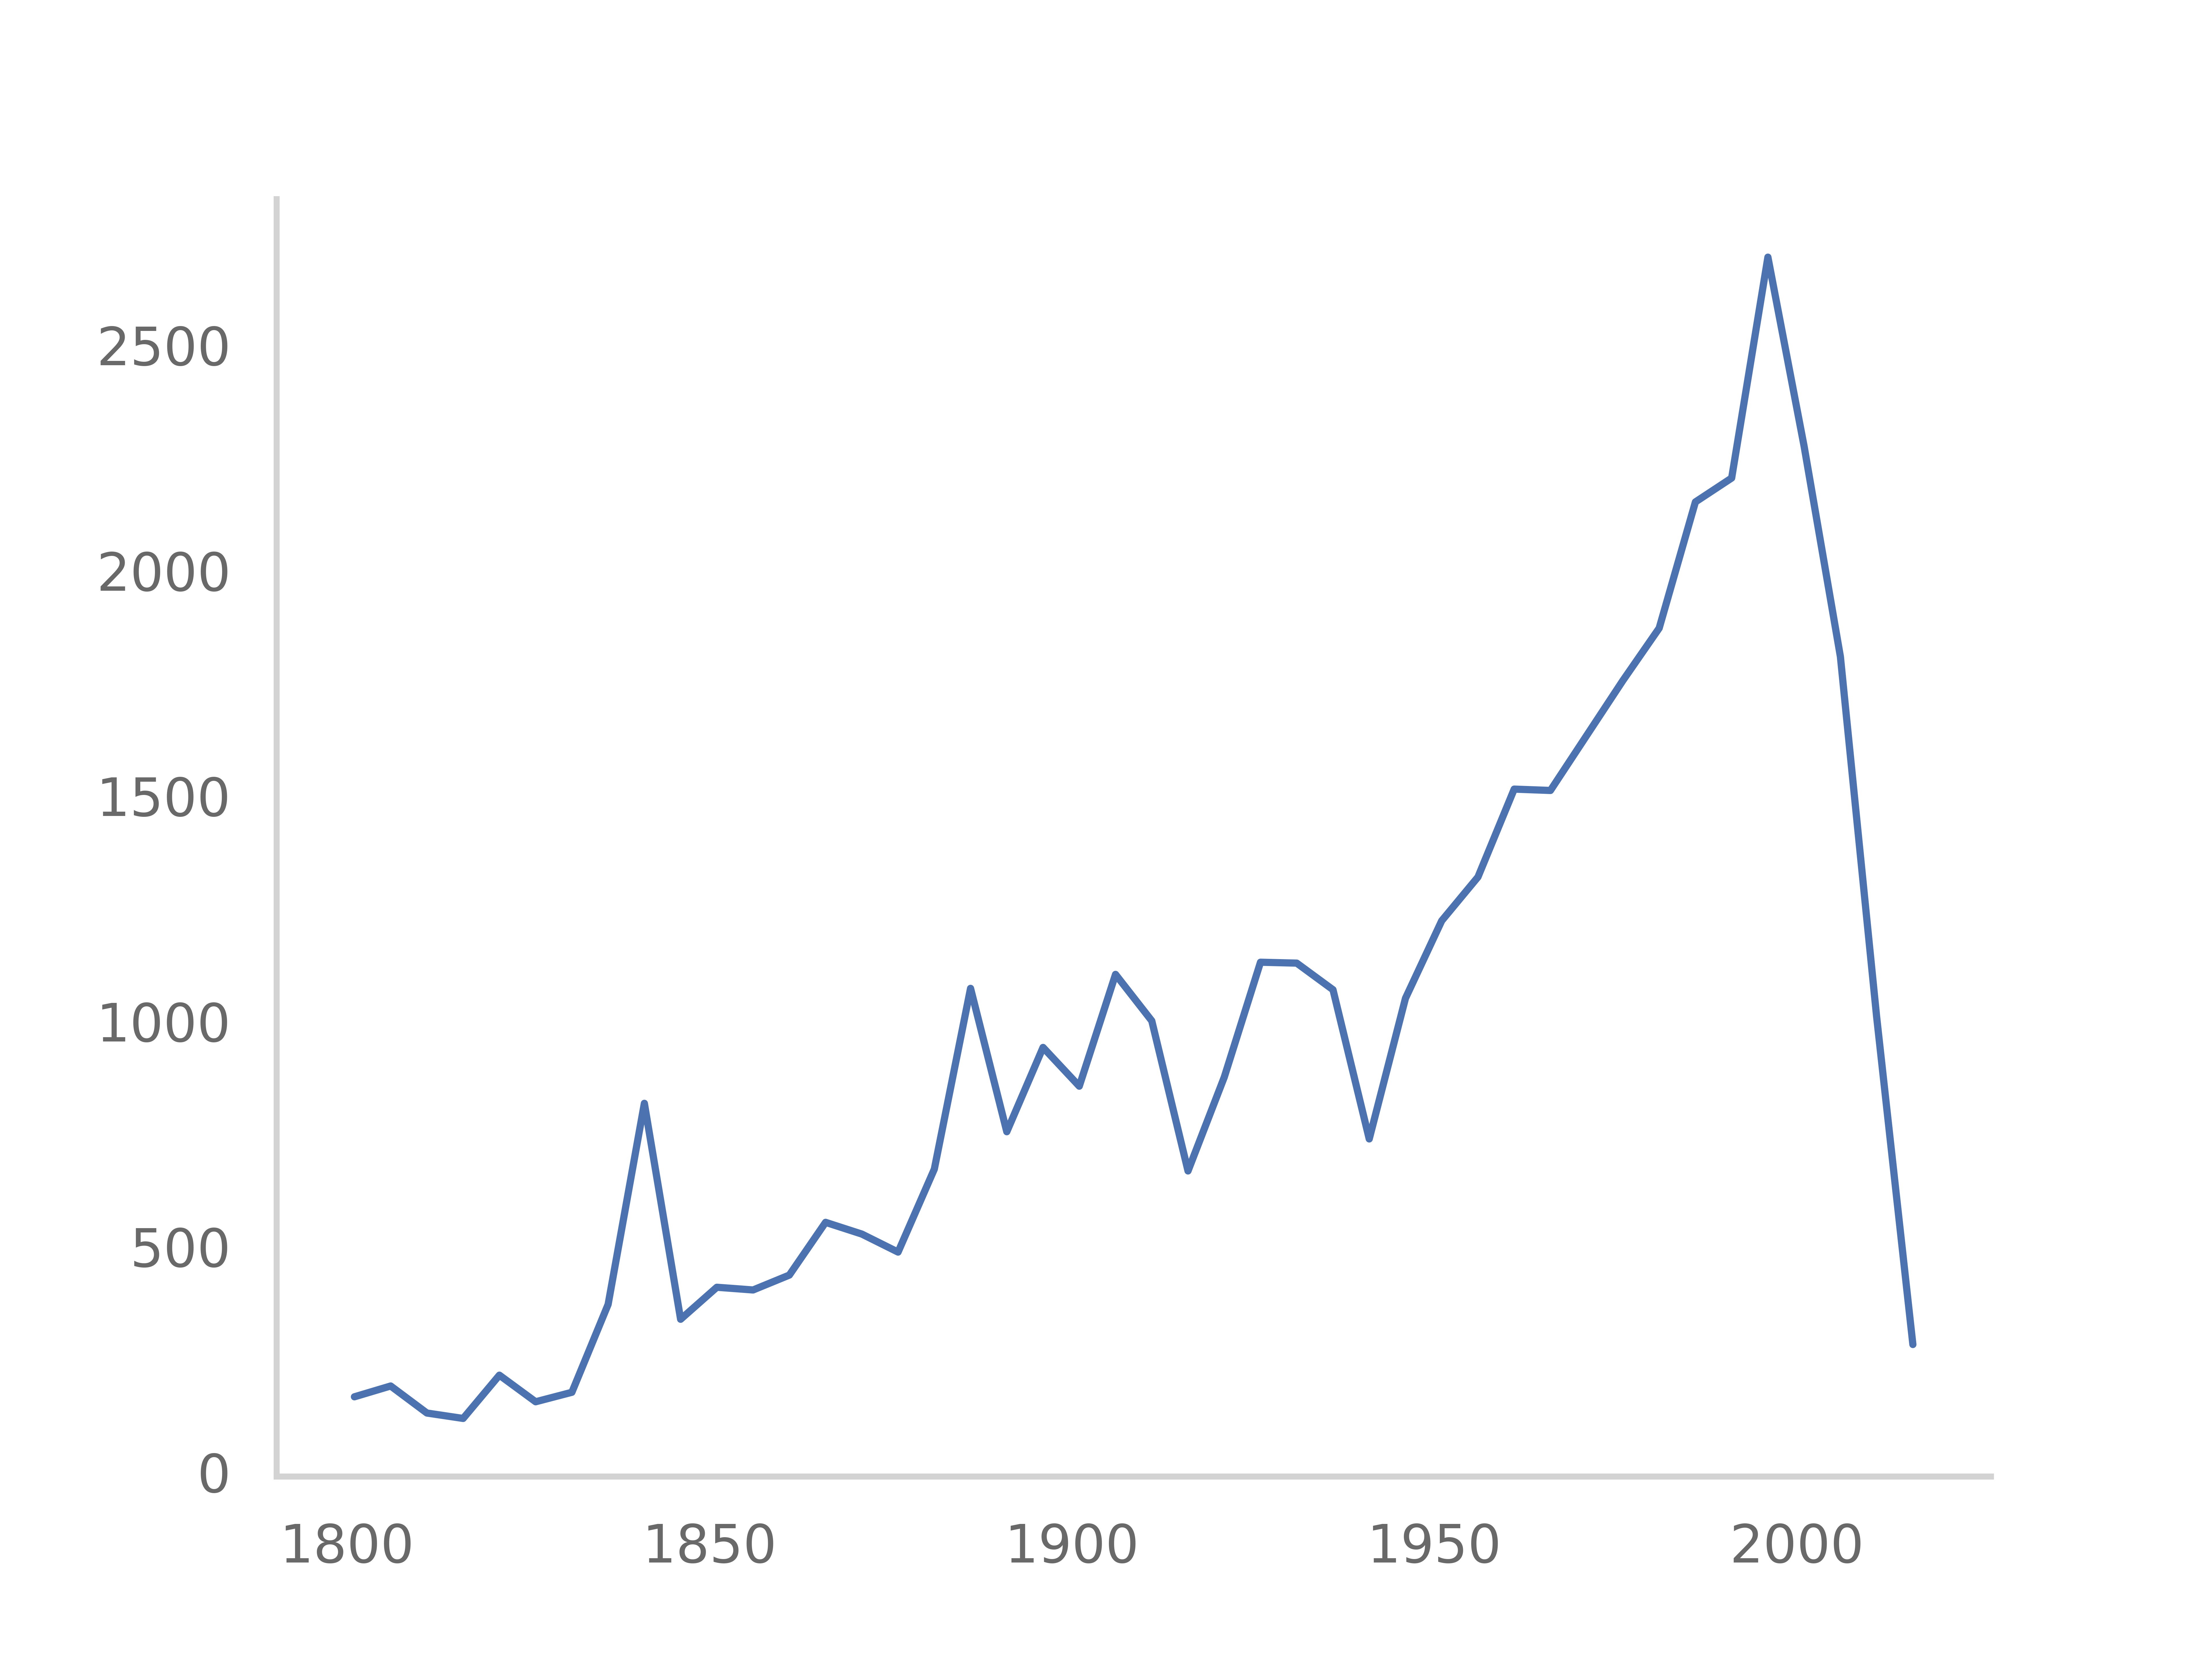
\includegraphics[width=0.8\linewidth]{invasion_per_year}
		\caption{Number of invasion per year.}
\end{figure}
\end{frame}

\begin{frame}
	
	\begin{itemize}
	\item 	They are a threat to biodiversity.
	\item 	The economic impact of alien species in Europe is estimated to be close to 13 billion dollars annually.	
	\end{itemize}		
\end{frame}

\begin{frame}
	We are interested in studying the dynamics of co-invasion of alien species.	
\end{frame}

\begin{frame}
	\frametitle{The Alien Species First Records database}
	
	The dataset contains the years of the first establishment of alien species in regions worldwide. To date is the most exhaustive source of first records of alien species currently available
	
	\bigskip
	
	The current version includes 61,751 invasions of 23,191 species divided into 18 taxonomic families in 276 regions ranging from 7000 BC to 2020 AD. 
%It's worth mentioning that regions can be countries, islands etc	
\end{frame}

\begin{frame}
The most abdundant families are Vascularp Plants and Insects.

\begin{figure}
		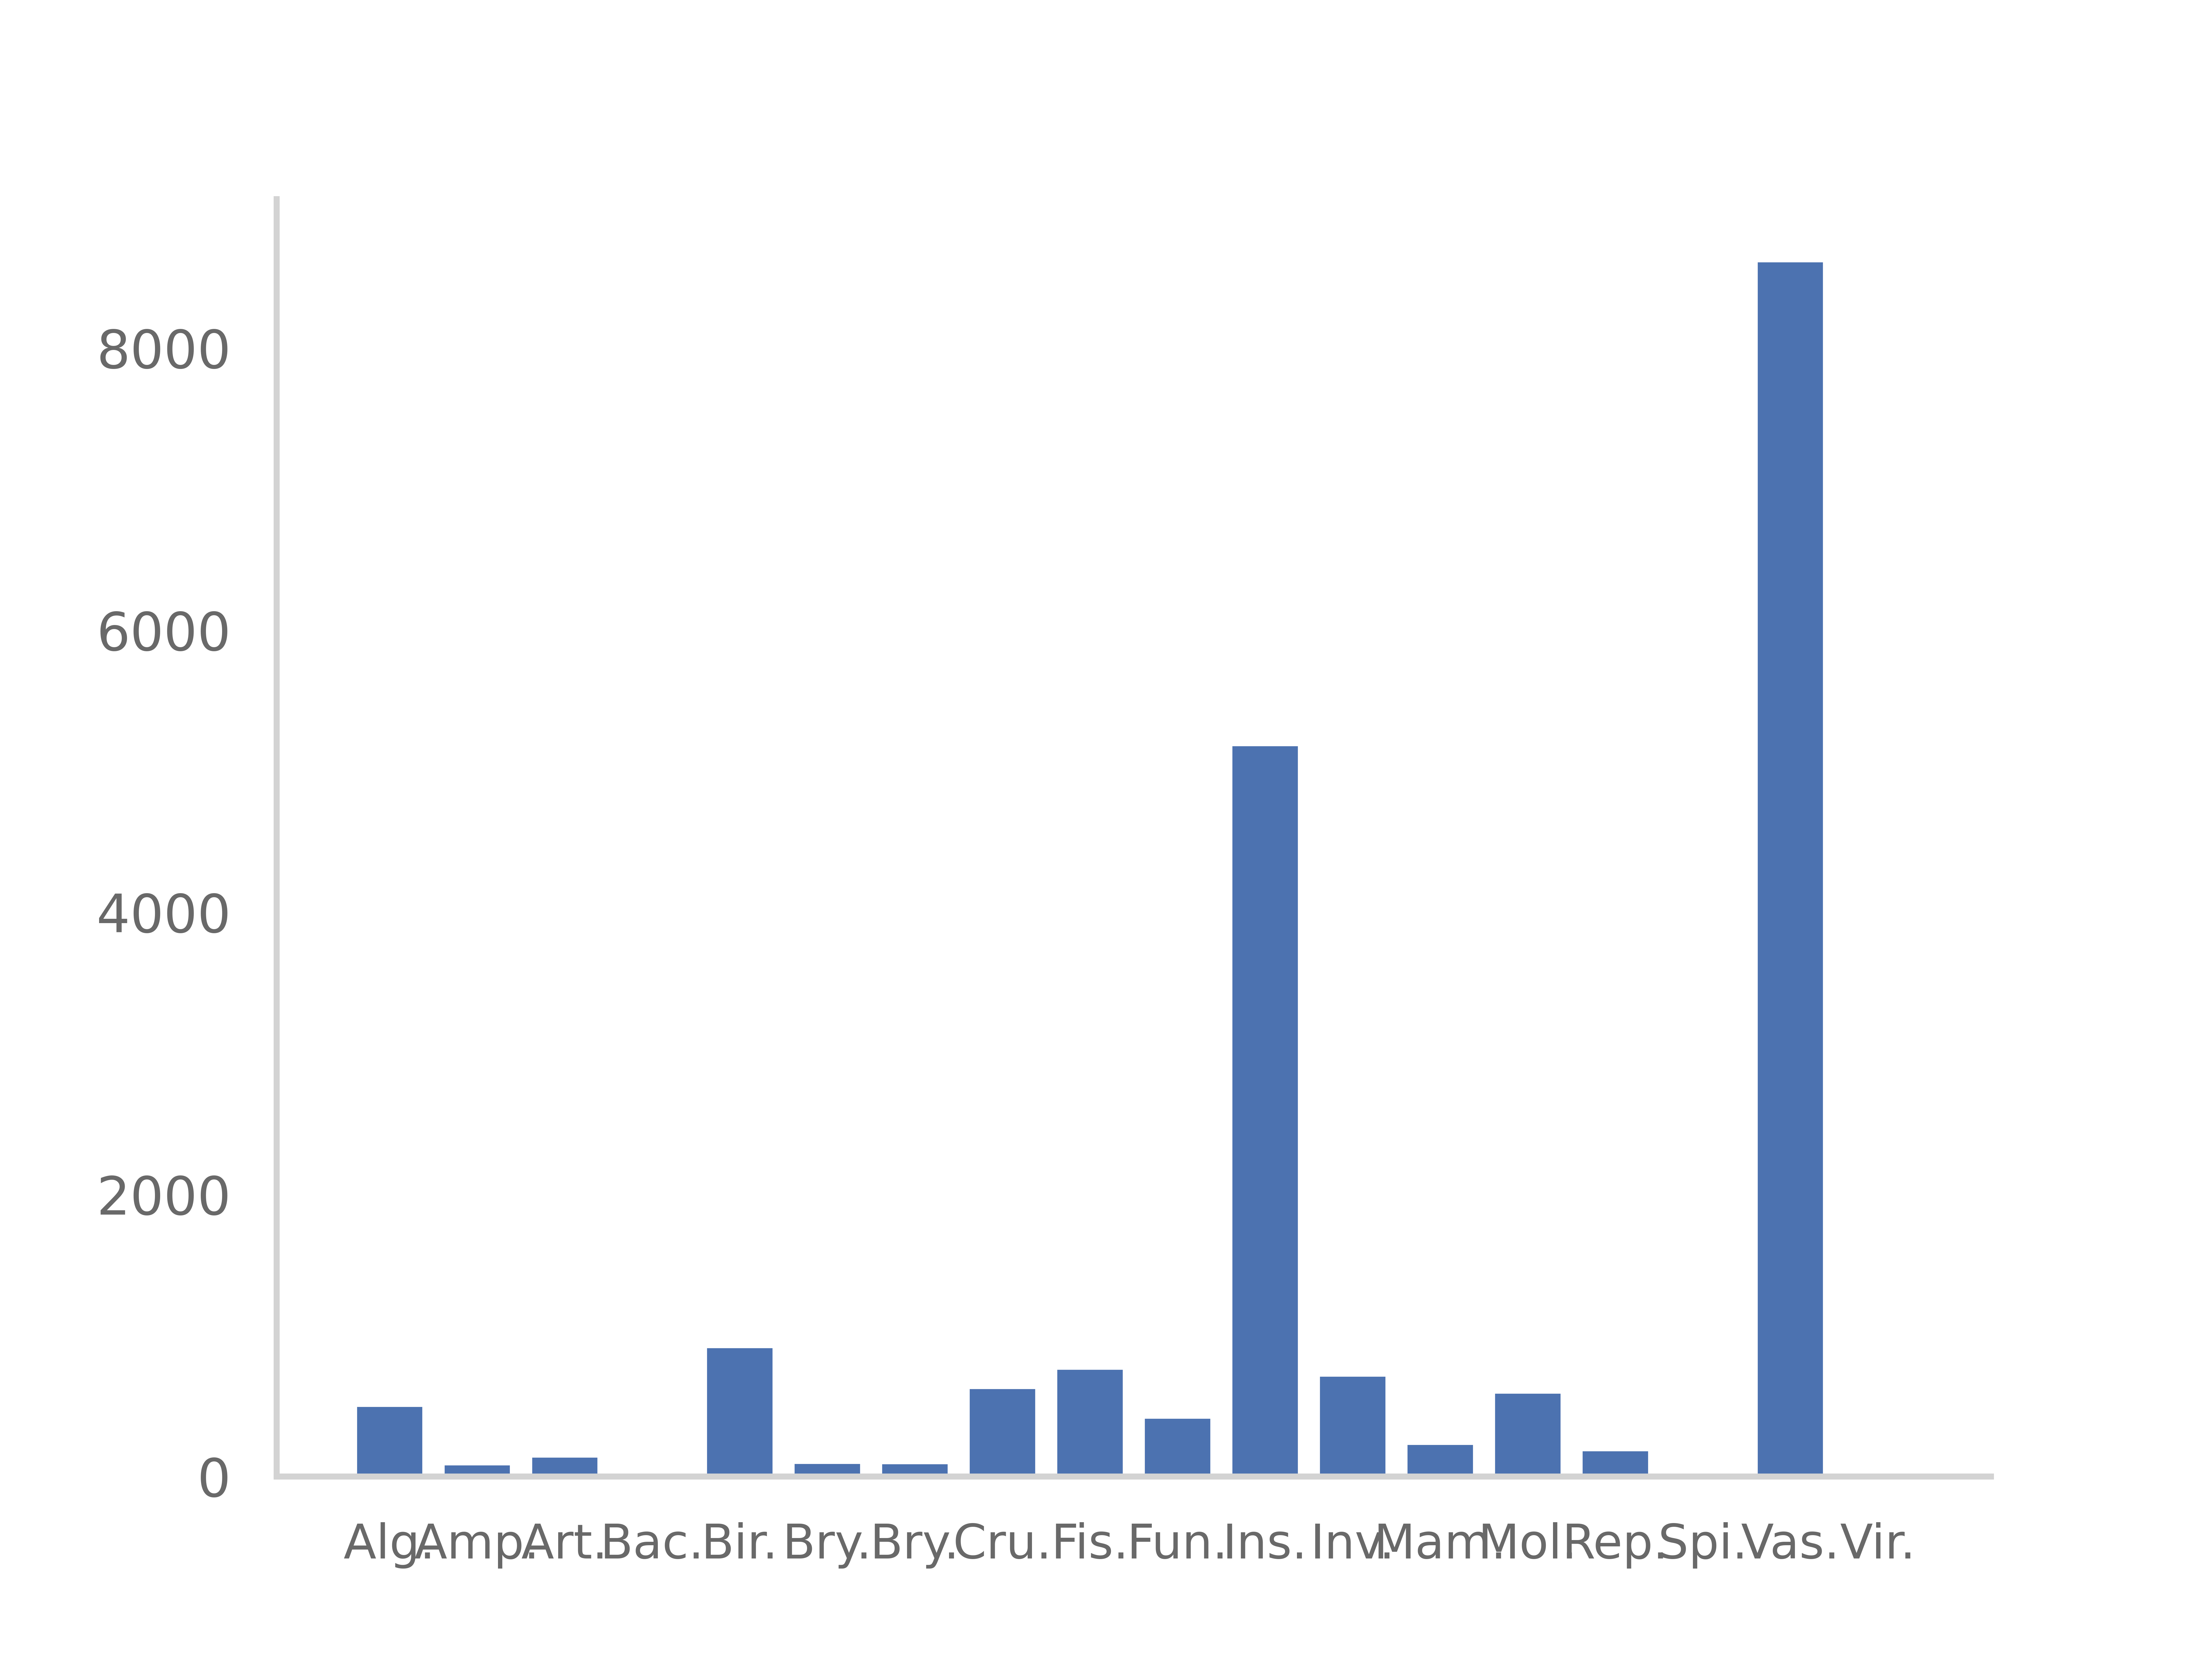
\includegraphics[width=0.8\linewidth]{histogram_taxfam}
		\caption{Number of species per taxonomic family.}
	\end{figure}
\end{frame}

\begin{frame}
		
	We focus our research in the timeframe lasting from 1850 to 2010 to ensure reliability and trustiness of the dataset.

	
	\smallskip
		
	\begin{figure}
		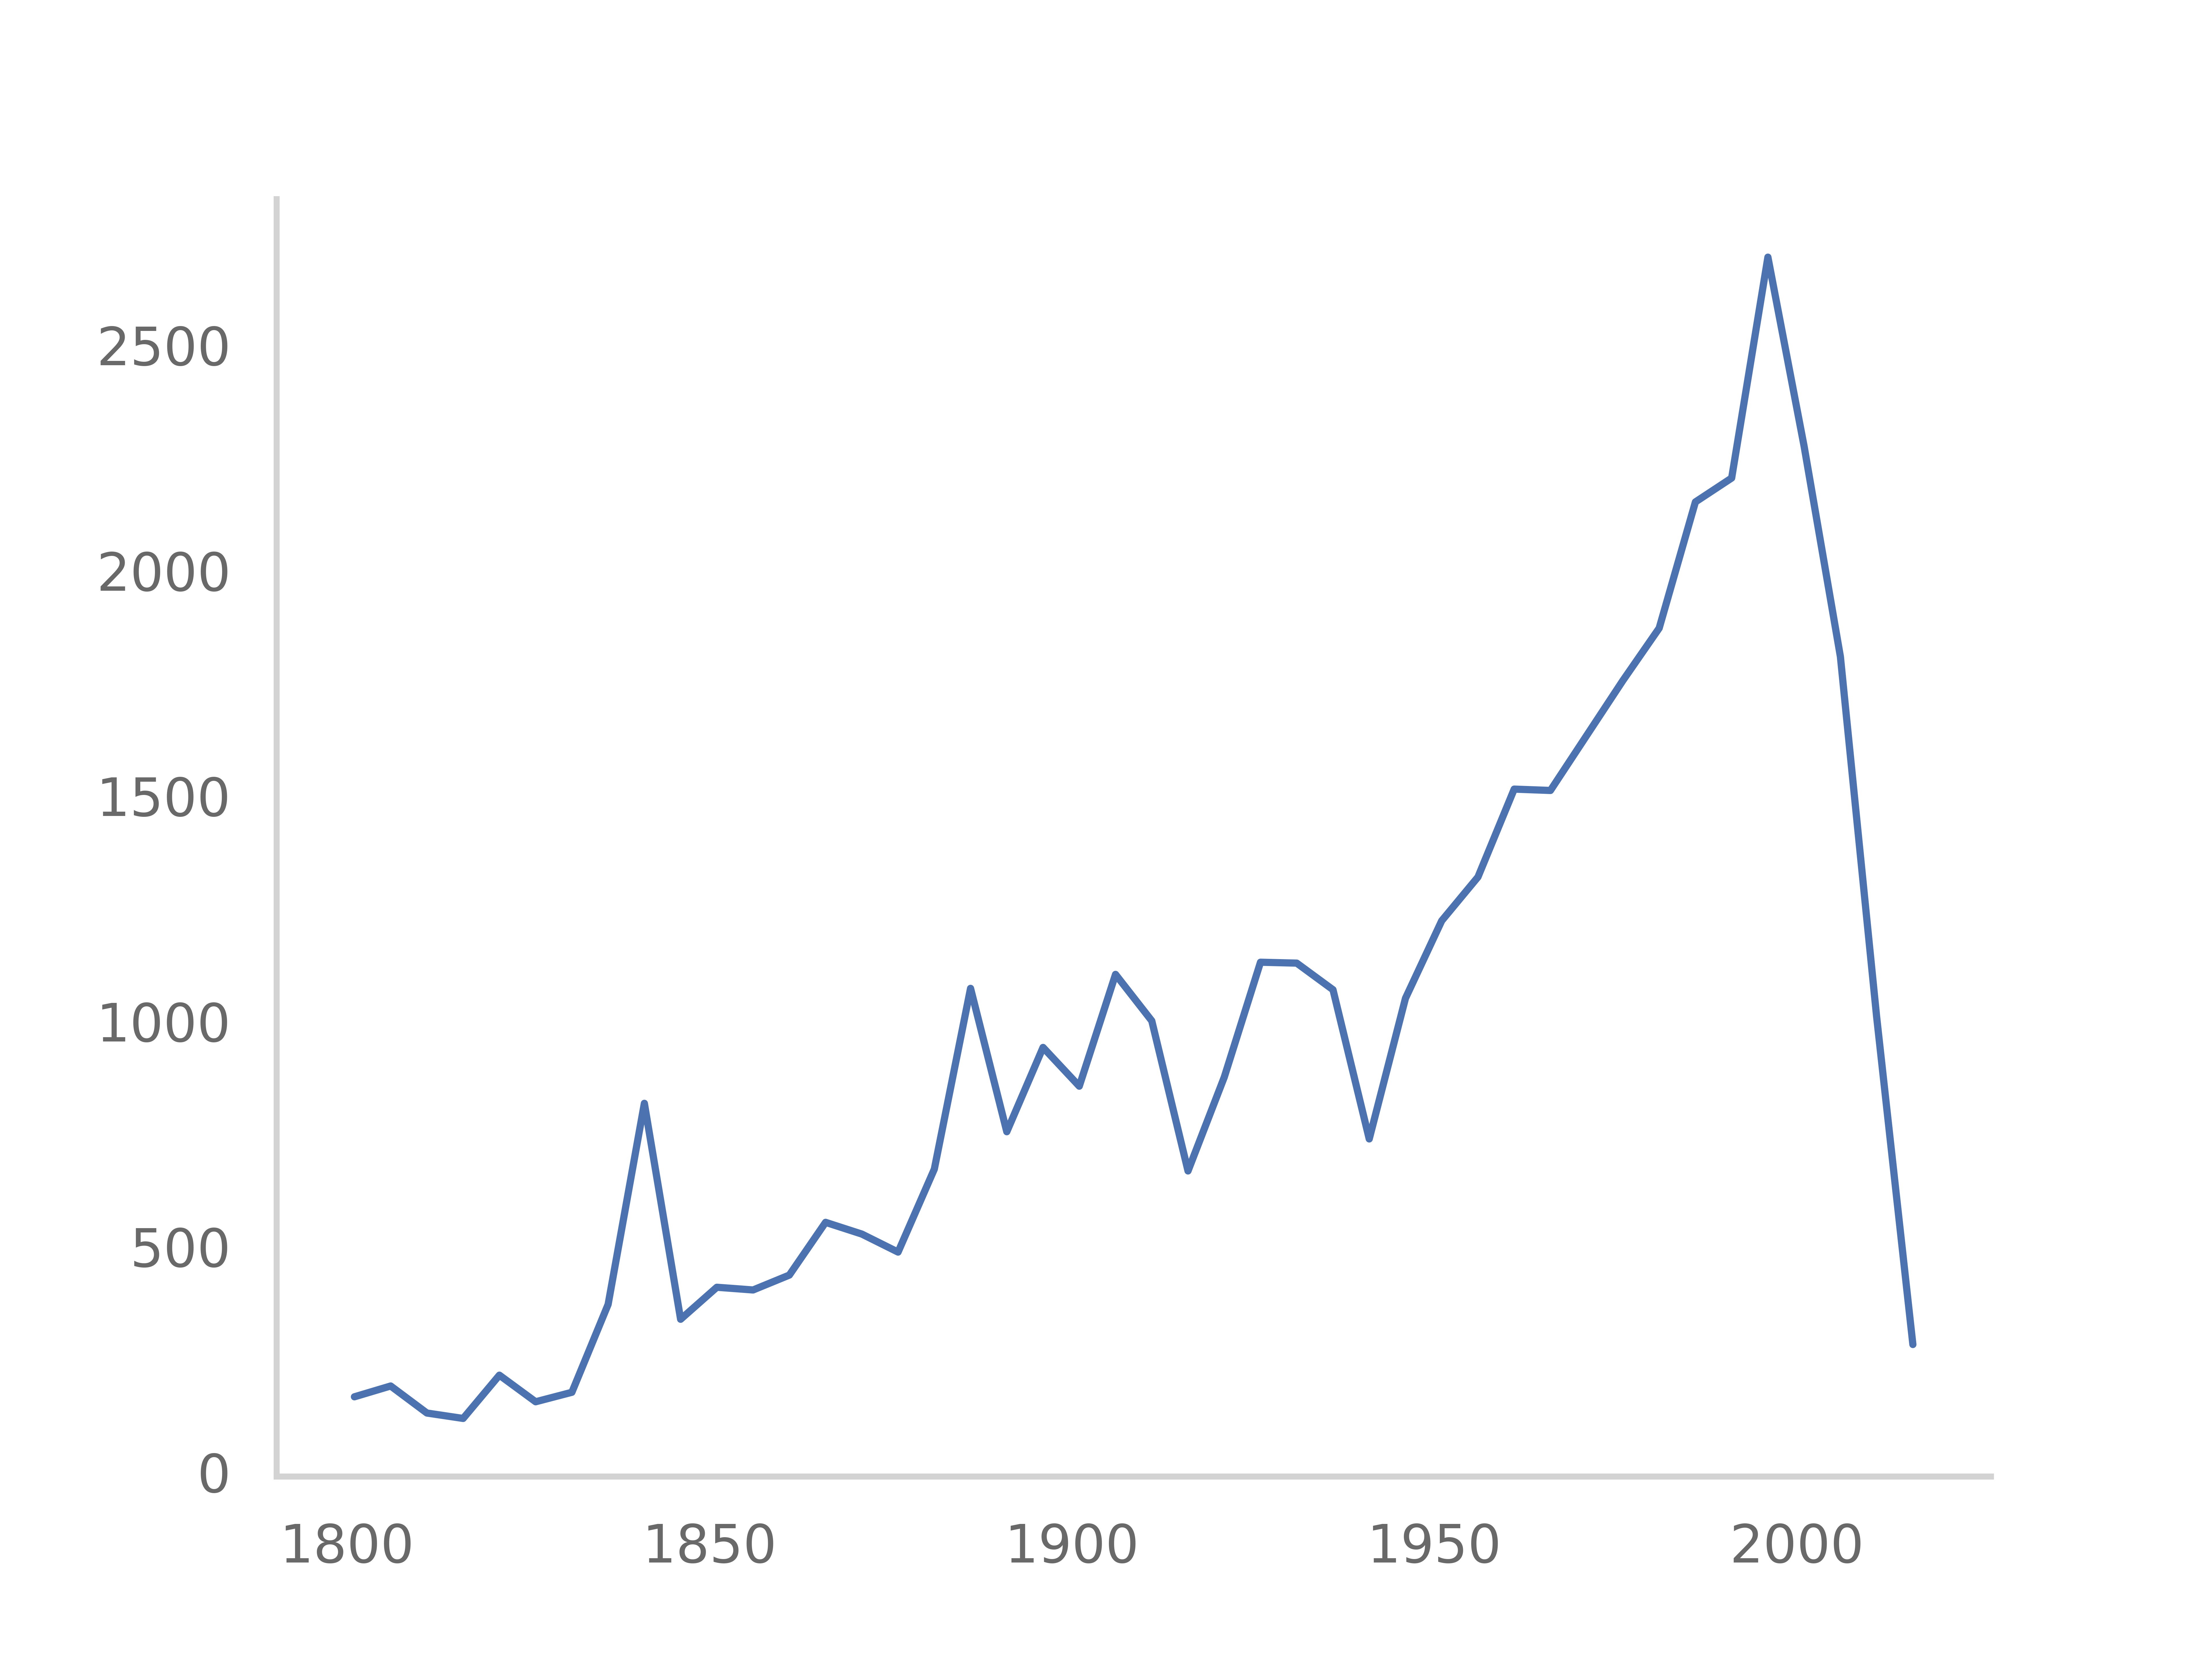
\includegraphics[width=0.6\linewidth]{invasion_per_year}
		\caption{Number of invasion per year.}
	\end{figure}
	
	\smallskip	
\end{frame}

\subsection{Dataset spatial complexity}
\begin{frame}
	\frametitle{Spatial complexity and dataset sparsity}
	Taking into consideration all taxonomic families, this timeframes covers a total of $19390$ alien species. Unfortunately, this number of species is too large for our model requirements.

\end{frame}

\begin{frame}

	The peak number of invasions per year is close to 5000 invasions around the year 2000, with an average number of invasions per year during the study of about 2800. Considering this number of average invasions per year and the fact that there are more than 20’000 species the dataset is considered to be sparse.

\begin{figure}
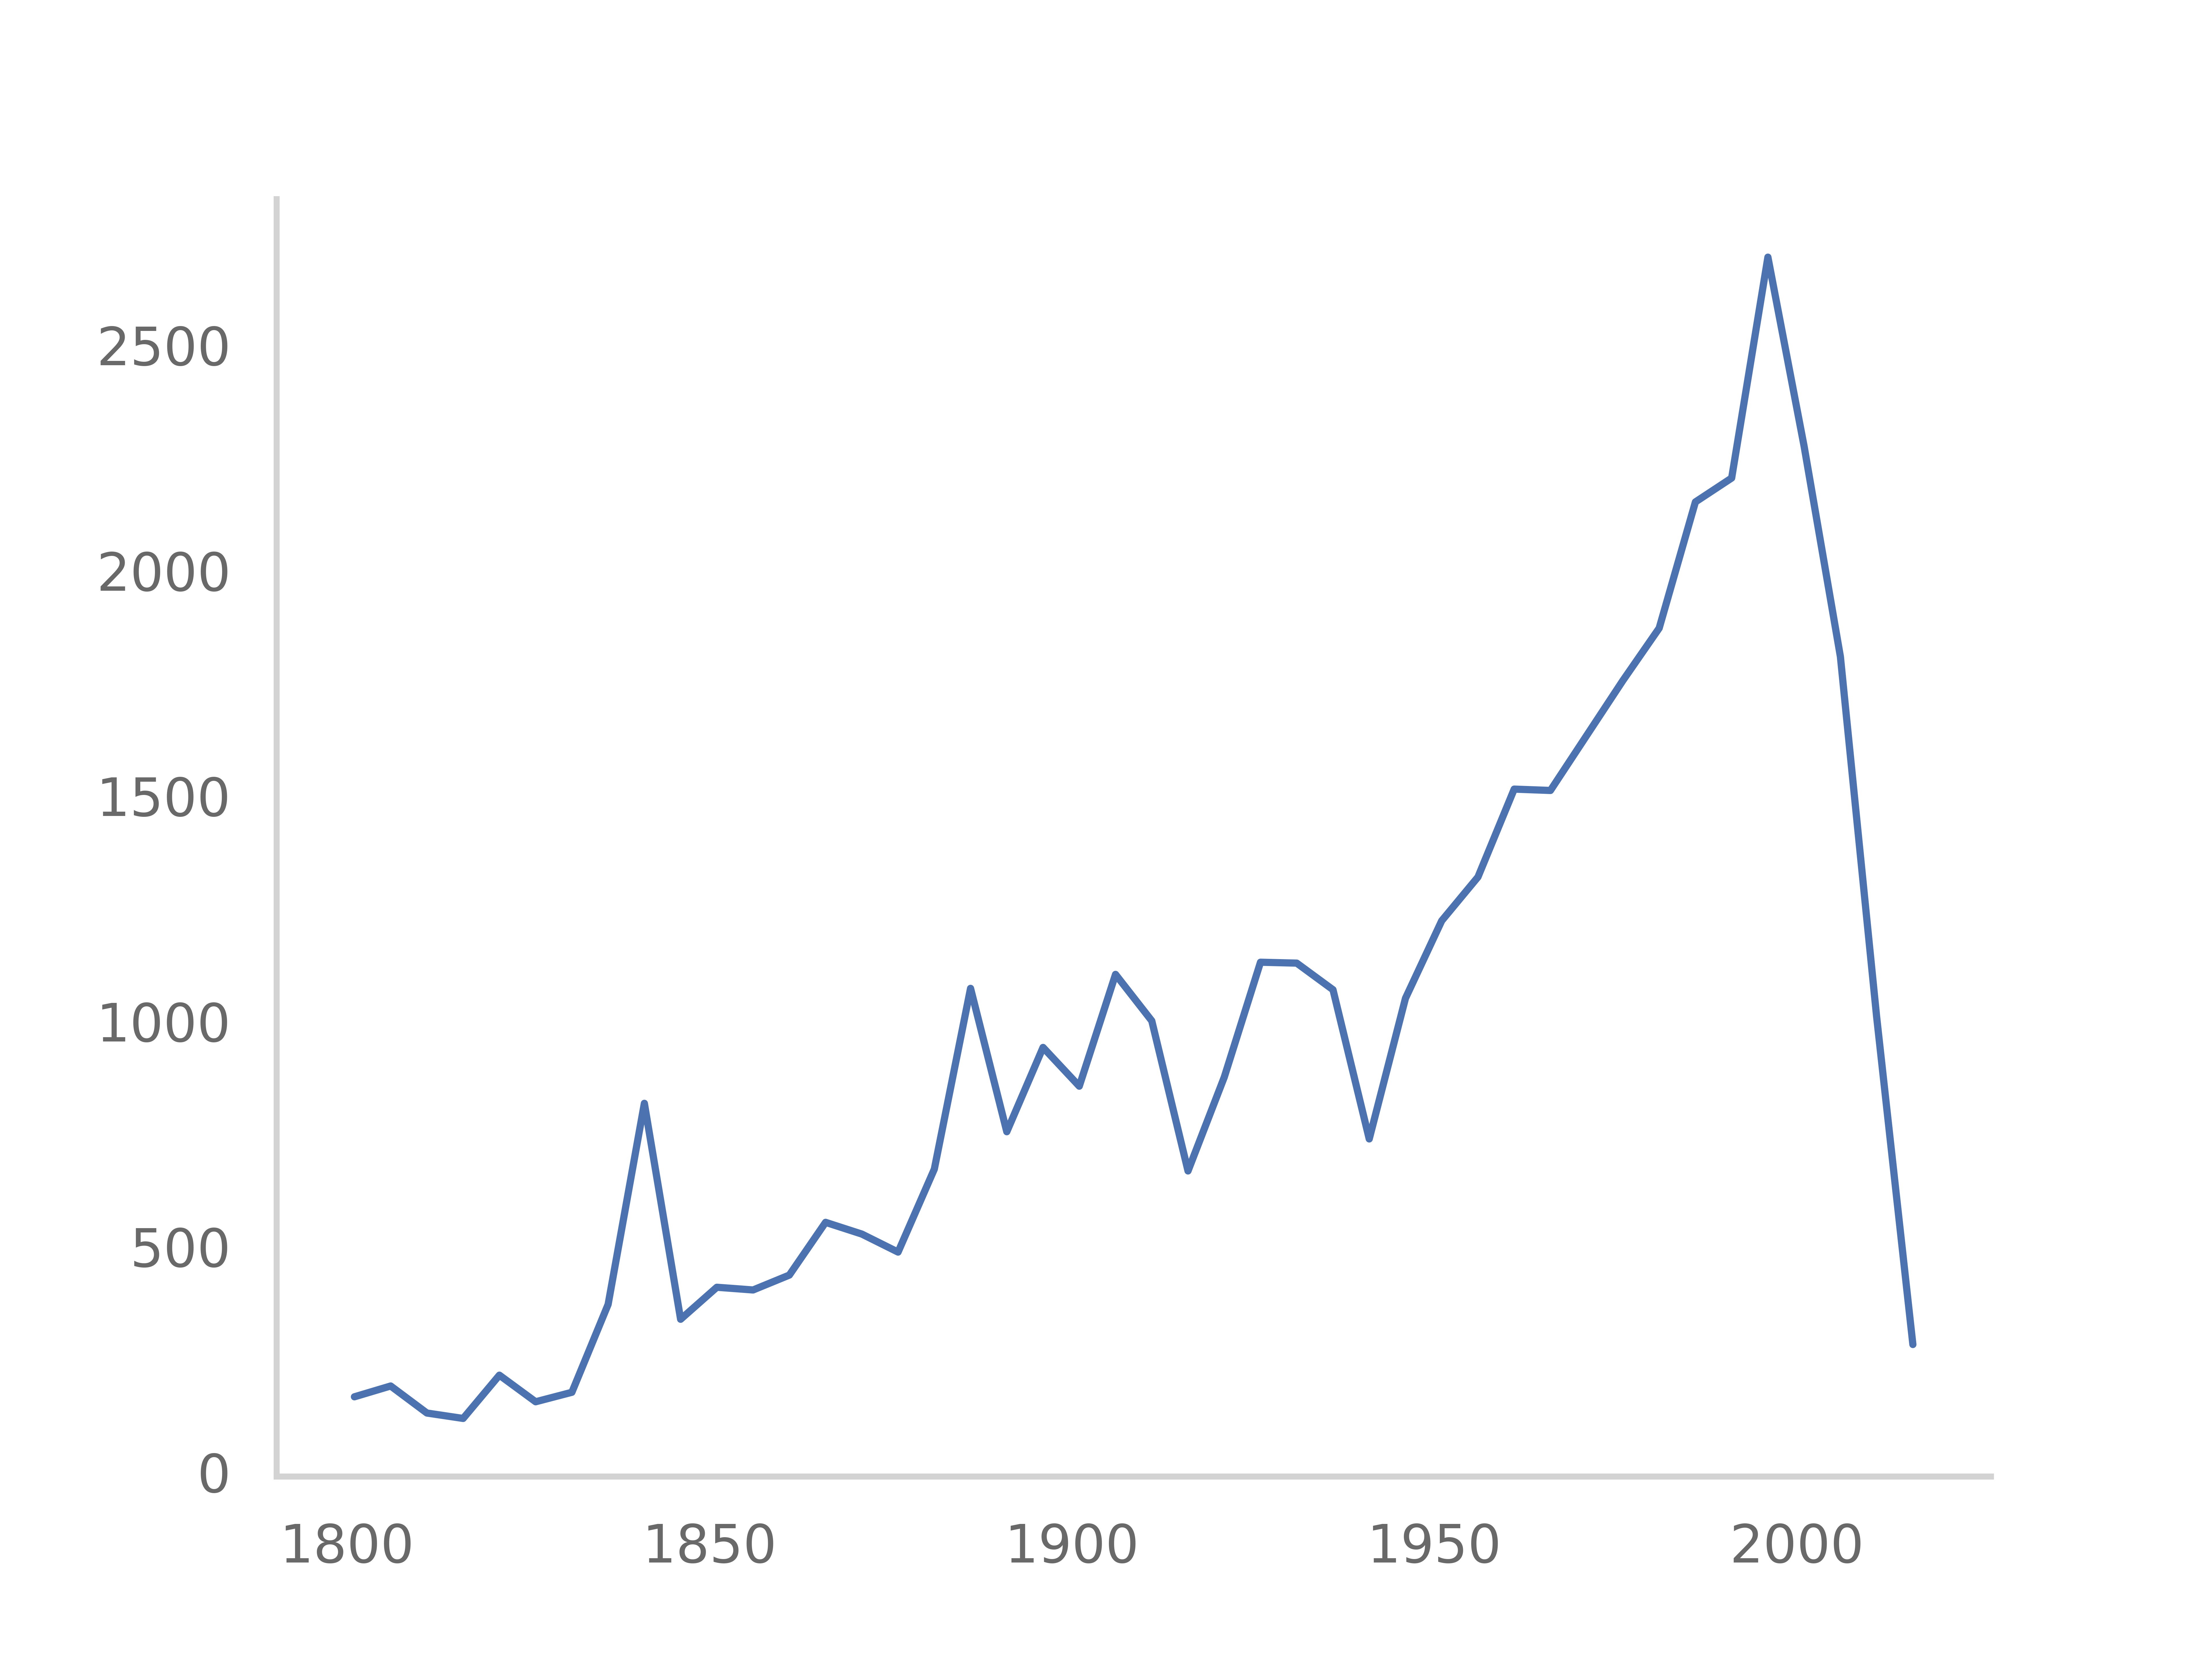
\includegraphics[width=0.5\linewidth]{invasion_per_year}
		\caption{Number of species per taxonomic family.}
	\end{figure}

\end{frame}

\subsection{Filtering the dataset}
\begin{frame}
	\frametitle{Filtering assumptions}
	To reduce the spatial complexity of the dataset we made the following two assumptions:
	\begin{enumerate}
	\item Remove all islands
	\item Remove all species that did not invade at least 5 regions
	\end{enumerate}
\end{frame}

\begin{frame}
\frametitle{Assumption 1: Remove islands}
We are mainly interested in the interactions between larger regions. Islands are not large enough to be interesting. 

\begin{figure}[H]
    \centering
    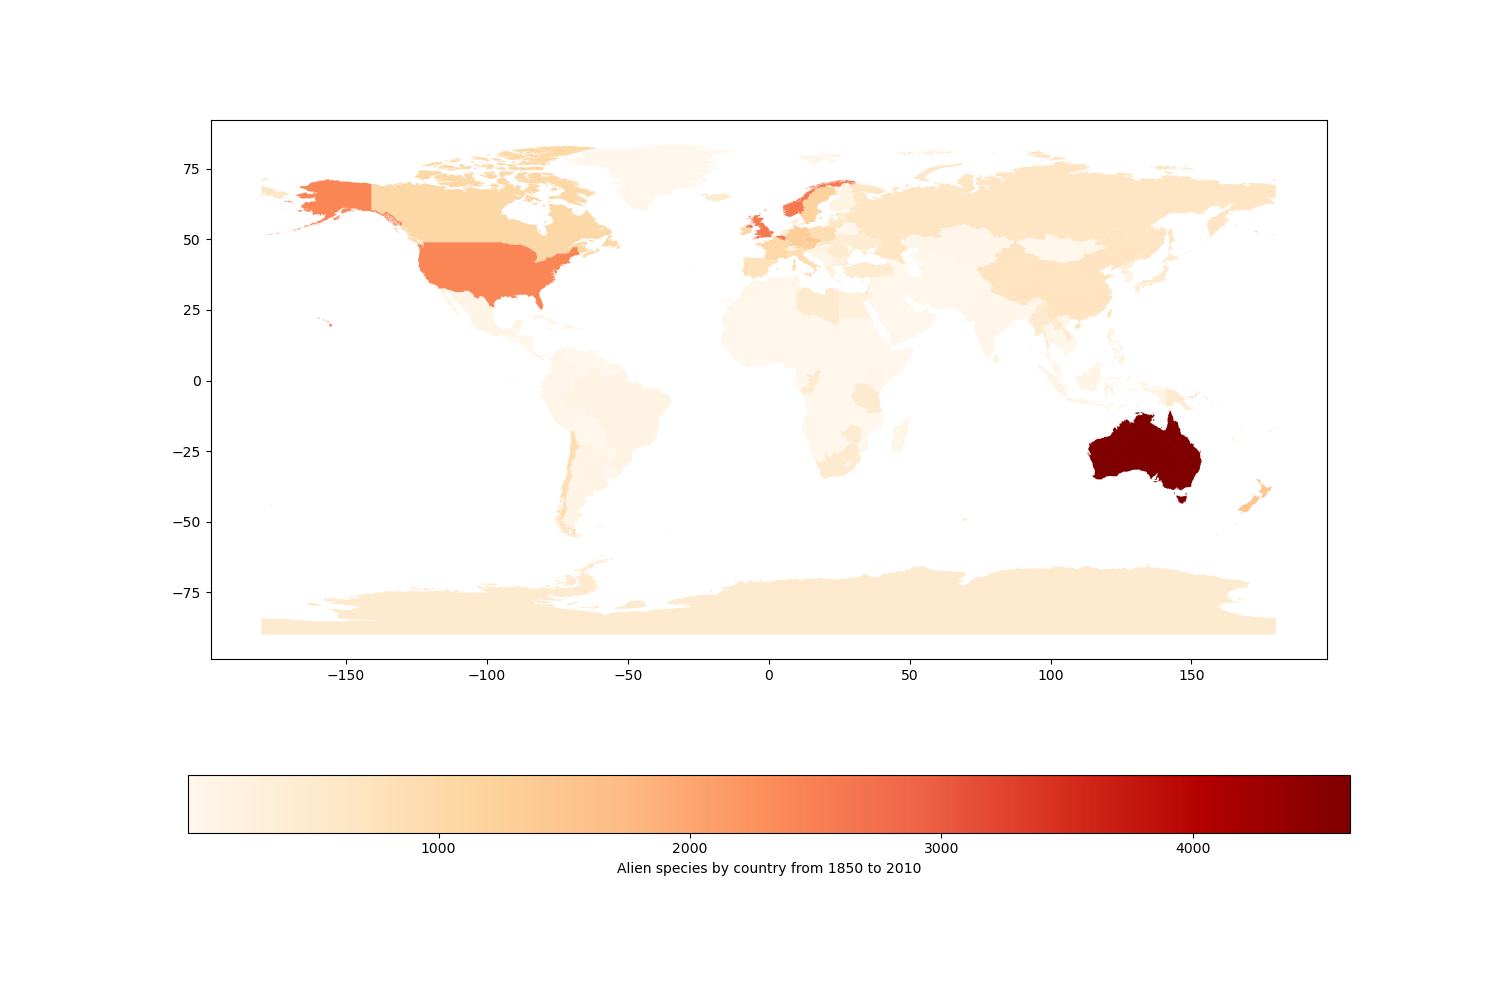
\includegraphics[width=0.95\textwidth]{region_invasion.png}
\end{figure}

\end{frame}

\begin{frame}
\frametitle{Assumption 2: Remove non-relevant alien species}
\begin{figure}
\centering
\begin{minipage}{.5\textwidth}
  \centering
    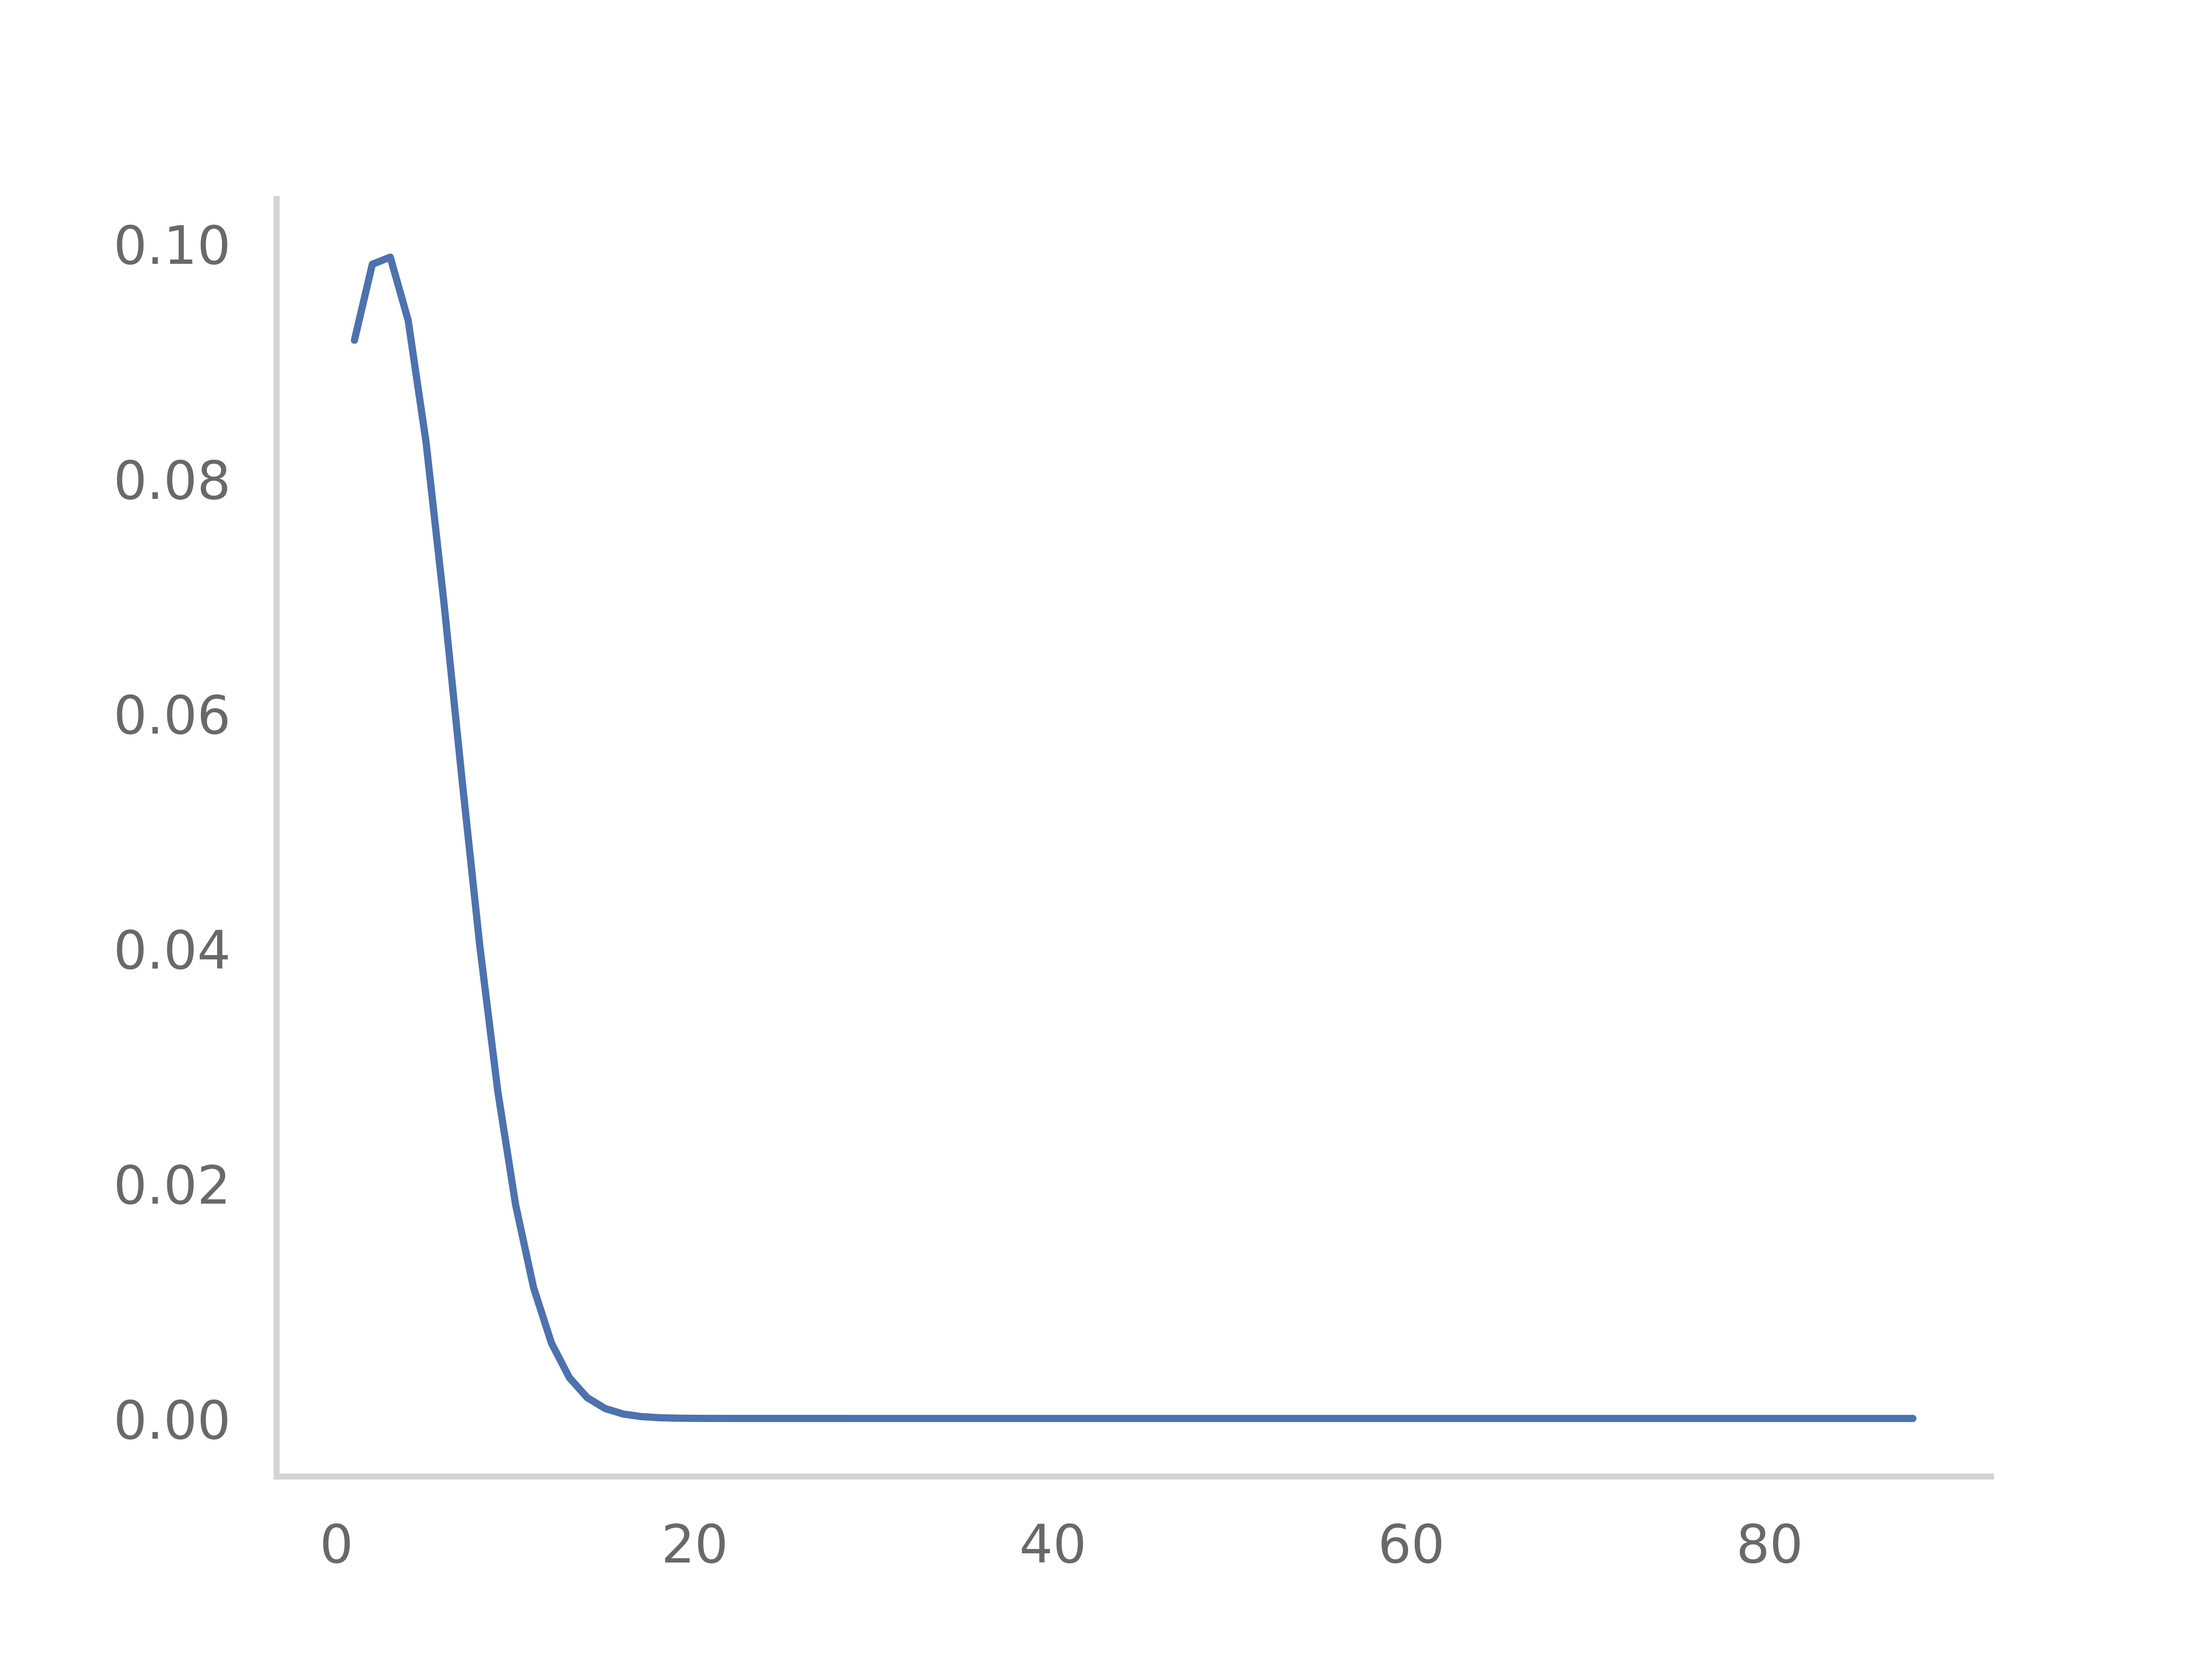
\includegraphics[width=0.85\textwidth]{species_region_invasion_no_filter.png}
%	\label{fig:pdf_invasions}
%    \caption{Probability density function of of the number of invasions.} 
\end{minipage}%
\begin{minipage}{.5\textwidth}
  \centering
    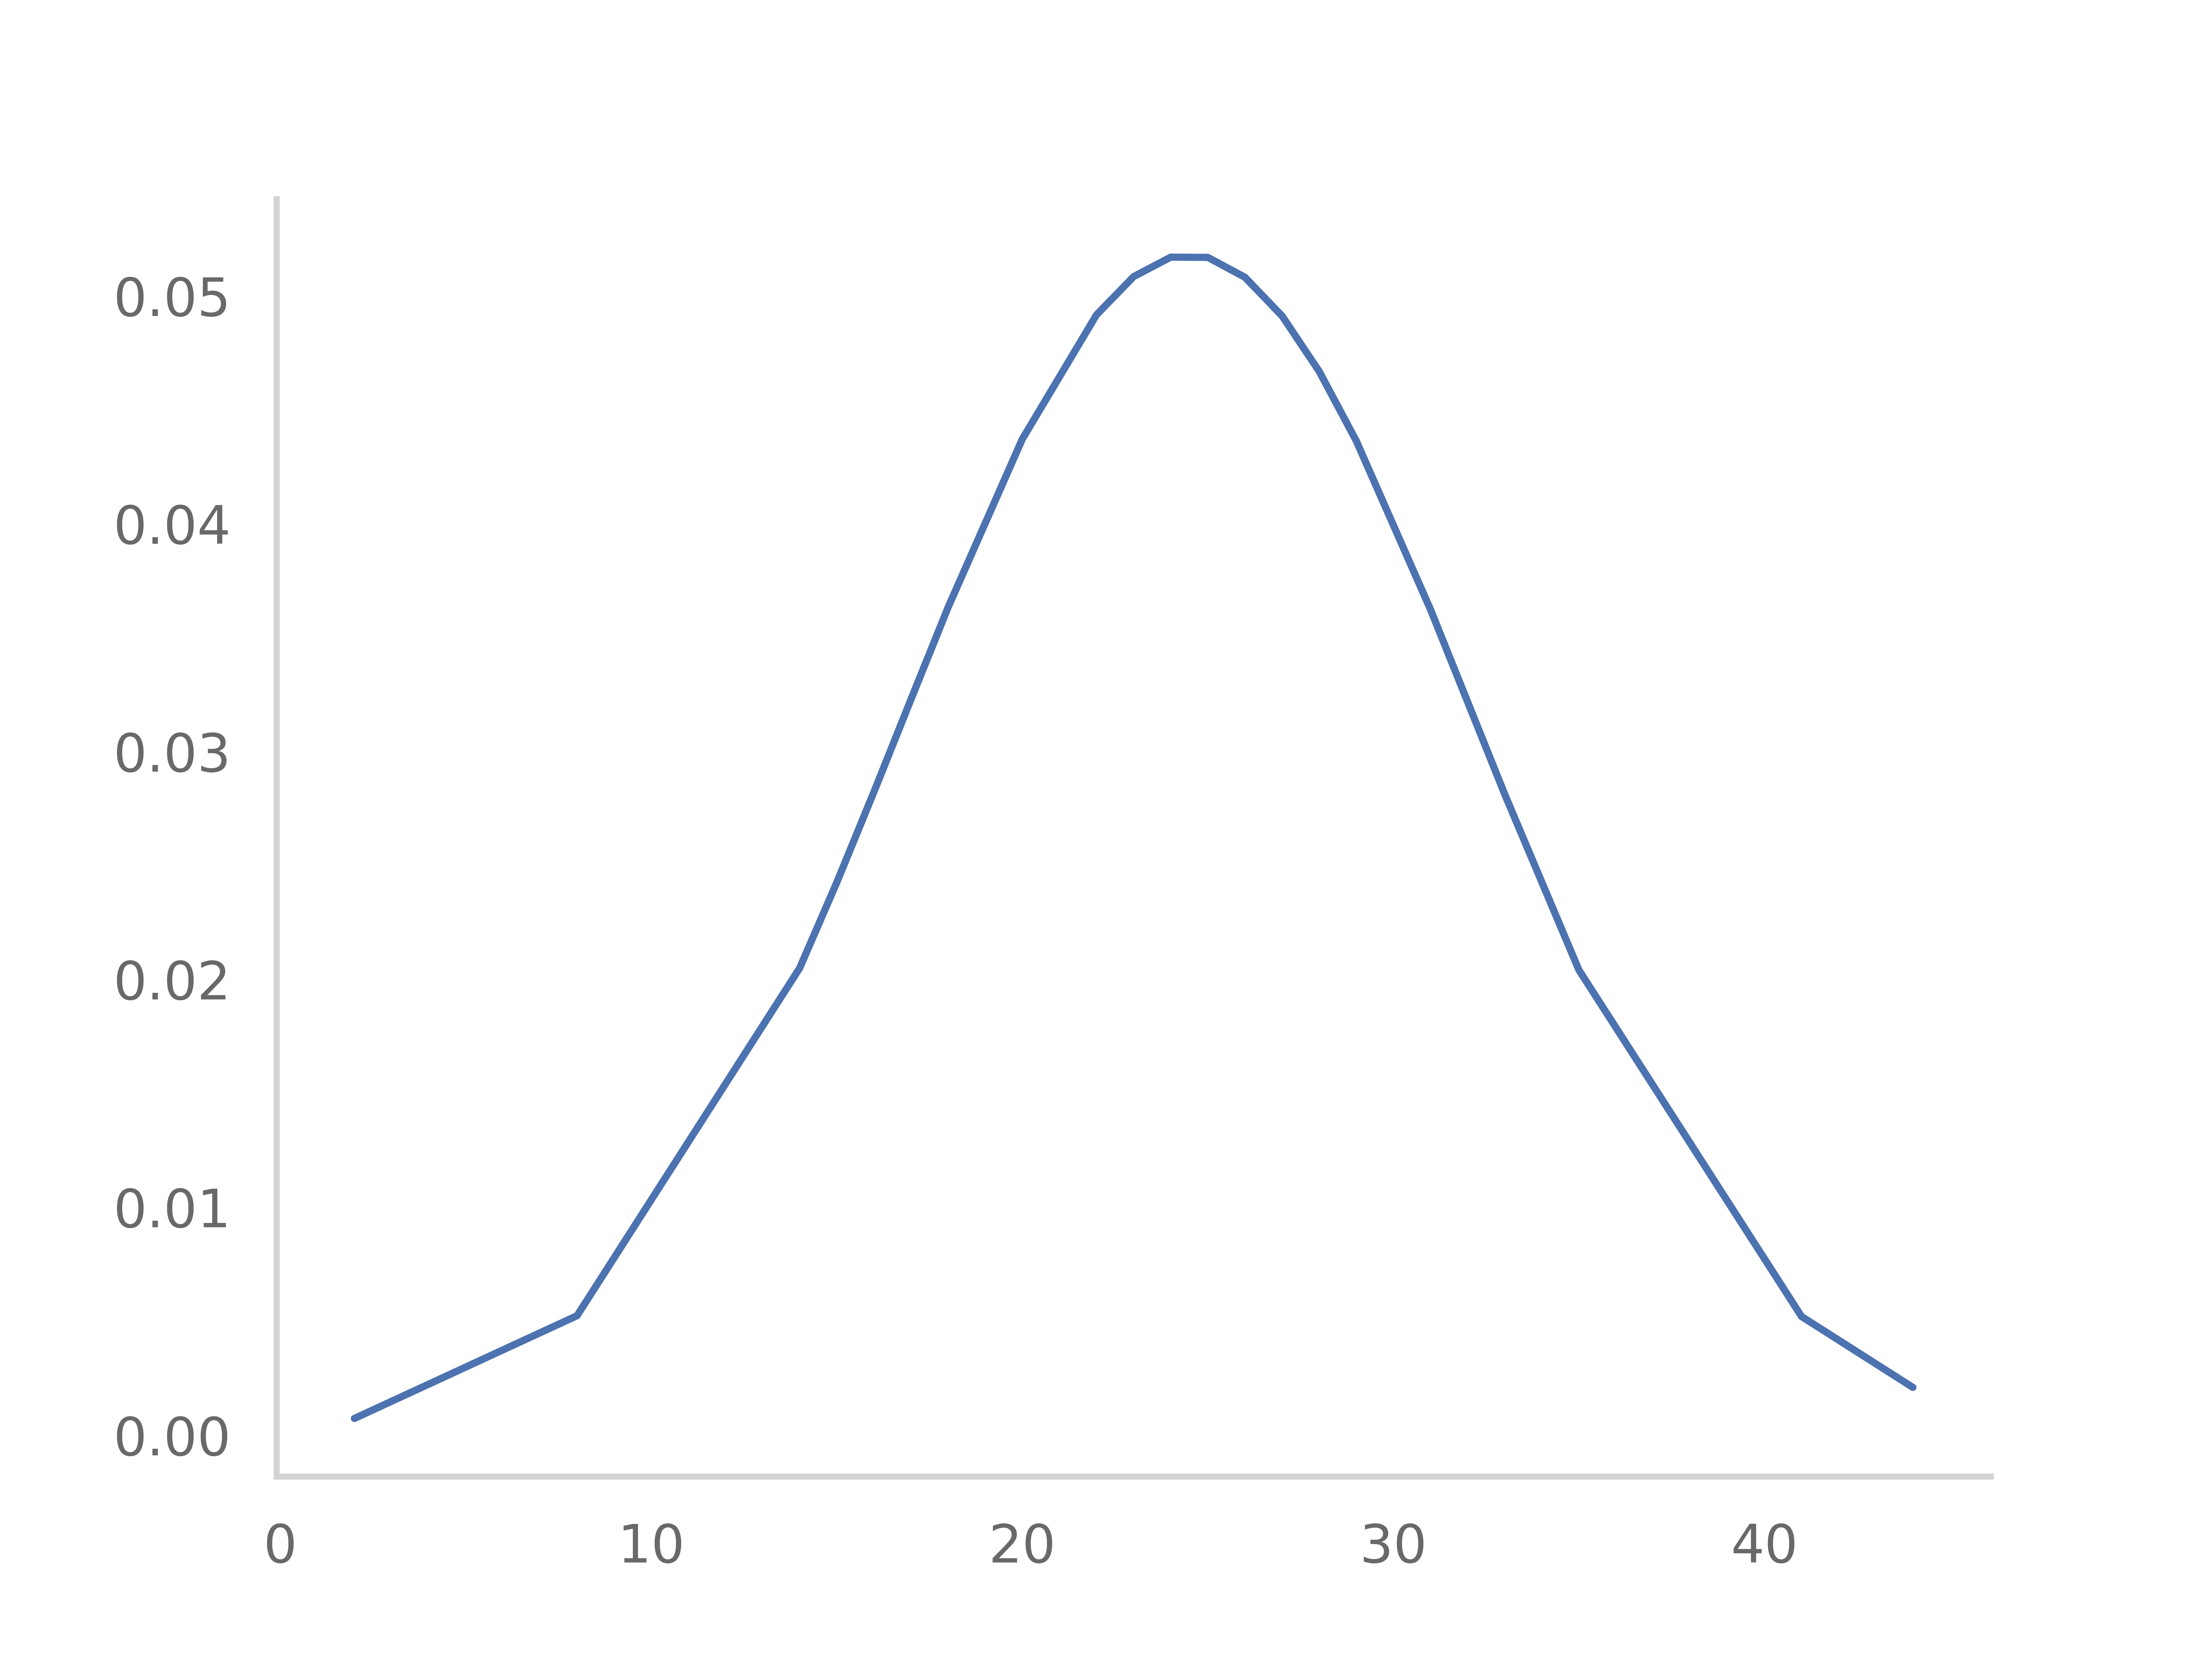
\includegraphics[width=0.85\textwidth]{species_region_invasion.png}
%    \label{fig:pdf_invasions_filtered}
%    \caption{Probability density function of of the number of invasions.}
\end{minipage}
\caption{Probability density function (PDF) of the number of invasions during the entire time frame of the study (1850-2010). The left graph shows that the PDF is strongly left skewed. The second PDF, on the right, is generated after removing all species that did not invade a significant amount of regions.}
\label{fig:pdf_invasion}
\end{figure}

\end{frame}


\begin{frame}
Under these two assumption, we focused our research on $1724$ species and $153$ regions in $15947$ invasions from $1850$ to $2010$.
\end{frame}

% Model section 10 minutes
%------------------------------------------------
\section{Model}
\begin{frame}
	\frametitle{Relational Event Model (REM)}
	
%	\begin{definition}
%		A \alert{prime number} is a number that has exactly two divisors.
%	\end{definition}
%	
	
	A relational event is an interaction between a sender and a receiver at a specific timestamp. An invasion of a species into a region can be described as a relational event. A relational event model (REM) studies the temporal sequence of such relational events.
\[
e_i = (s_i, r_i, t_i)
\]	
	
	This framework has many advantages in the fact that it is able to study underlying temporal patterns, can efficiently deal with time-varying variables and it is an extremely adaptable hypothesis testing tool.
	
However, due to the high number of possible local network configurations, it is really hard to keep track of the past configurations to study dynamic networks.
\end{frame}

\begin{frame}
The risk set $\mathcal{R}_t$ is the set of all dyads for which, at a given timestamp $t$, a relational event can occur,

\[
\mathcal{R}_{t} = \{(s,r) \; | \; \textrm{may occurs} \; \textrm{at} \; t_i\}
\]

We assume the waiting time $T_{s,r}$ for a particular dyad to happen between a species $s$ and a region $r$ is assumed to be exponentially distributed 

\[
T_{s,r} \sim Exp(\lambda(s, r, t) )
\]

with the hazard function $\lambda$ is defined as

\[
\lambda(s, r, t) = \lim_{\delta t \lim 0^+} \frac{P(t \leq T_{s,r} \leq t + \delta t | t \leq T_{s,r})}{\delta t}
\]
\end{frame}

% Talk about the hazard function 
\begin{frame}
Every invasion of a species $s \in S$ and region $r \in R$, where $S, R$ are respectively the sets of species and regions in the dataset, can be modelled as a multivariate Poisson counting measure  $N$.

\[
N_t(s, r) = \textrm{number of invasions of} \; s \; \textrm{in} \; r \; \textrm{in the interval} \; [0, t]
\]

An alien species is not allowed to leave a region after an invasion has happened and, eventually, invade it a second time. Therefore, an invasion can happen only once. The counting process $N$ is therefore bounded by 1.
\end{frame}

\begin{frame}
	\frametitle{A latent space relational event model}
	We dispose species and regions into a latent space $X \in \mathcal{R}^n$. Each actor is assigned a position inside $X$.
	
	\bigskip
	
	By disposing of the species-region interactions in a latent space we "summarise" their configuration history hence we can effectively approximate the past information and train a REM more efficiently.
	
\bigskip
\begin{equation*}
    \begin{cases}
      x_k = x_{k-1} + \epsilon \; , \quad \textrm{where} \; \epsilon \sim N(0, \Sigma) \\
      y_k \sim Poi(\lambda_k) \;
    \end{cases}\,.
\end{equation*}

\end{frame}


\begin{frame}
The observed counts $y$ are a result of the dynamics of the actor's positions and interactions in the REM and latent space $X$. The stochastic intensity of the counting process $N$ is modeled by the function $\lambda$. Heuristically, we assume that the rates $\lambda$ are functions of the distance between species $x_s(t)$ and regions $x_r(t)$ in the latent space. 

\bigskip

\[ \lambda^{s, r, k} = exp\left(\alpha-dist(x_s(k), x_r(k)) \cdot \lambda_1(k) \right) \cdot I \]

\end{frame}


\begin{frame}

\begin{itemize}
\item The position $x$ of each vector in the latent space $X$ is constrained by the distance to all the other vectors inside $X$.
\item The distance in this space represents an affinity of each species $s$ to create a connection to a region $r$ in the REM.
\item The structure of the latent space is driven by the similarity of nodes.
\item We are interested in studying the structure of $X$ and infer on the co-invasion of species.
\end{itemize}

%The position $x$ of each vector in the latent space $X$ is constrained by the distance to all the other vectors inside $X$. The distance in this space represents an affinity of each species $s$ to create a connection (i.e. to invade) a region $r$ in the REM. The structure of the latent space $X$ is therefore driven by the similarity between the nodes $s, r$. We expect species that tend to co-invade the same regions to be close in the latent space. Analogous, regions invaded by the same group of species should be near. We are interested in studying the structure of the latent space $X$ to infer which group of species has the tendency to co-invade regions.

\end{frame}

%----------------------------------------------------------------------------------------
% 	INFERENCE
%----------------------------------------------------------------------------------------
\begin{frame}
\title{Inference}

We aim to maximise the marginal likelihood: 

$$\int_x L(\theta, \Sigma ; y, x) dx$$

\bigskip

However a direct maximization is not possible. To infer on the structure of the latent space $X$, and the parameters $\theta$  and $\Sigma$ we use the Expectation Maximization (EM) algorithm. 
\bigskip

\begin{algorithm}[H]
\While{not converged}{
 $\textrm{E-step:} \;  E_{x|y}[Q(\beta^{n}, \Sigma^{n}] $\;
 $\textrm{M-step:} \; \beta^{(n+1)} = \textrm{argmax}_{\beta} \;Q(\beta^{n}, \Sigma^{n})$
}
\end{algorithm}

%with $Q(\beta^{n}, \Sigma^{n}) = E_{x|y} \left( log(p(x, y | \beta^{n-1}, \Sigma^{n-1}) \right)$

\end{frame}

\begin{frame}
 By exploiting the natural formulation of our latent space model we can solve the computationally challenging E-step by means of a Kalman filter by approximating the quantity $Q$ in function of its first two conditioned moments $E$, $V$. 
\end{frame}

%--------------- Maybe too in details?
%\begin{frame}
%By assuming that a step in time in the latent state can be approximated by the conditional distribution 
%
%\[
%x_{k} \sim N( \hat{x}_k, \hat{V}_k)
%\]
%
%\noindent the predict step of the Kalman filter estimates the first two moments of $x_k$. 
%
%\[
%\hat{x}_k = E[\hat{x}^-_k]
%\]
%\[
%\hat{V}_k = V[\hat{x}^-_k]
%\]
%
%Where $\hat{x}^-_k$  is an a-priori distribution of the state $x$ at time $k$, given the knowledge of the previous state.
%\end{frame}
%--------------- Maybe too in details?


\begin{frame}

\begin{algorithm}[H]

\textbf{Initialize: }
\begin{substeps}
$\hat{x}_0 = \mu_0 = E[x_0]$ \;
$\hat{V}_0 = V_0 = E[(x_0-\hat{x}_0)(x_0-\hat{x}_0)^T]$  \;
\end{substeps}
\For{k=1,...,n}{
  \textbf{Prediction step:}
  \begin{substeps}
	$\hat{x}_k^- = \hat{x}_{k-1} $ \;
	$\hat{V}_k^- =  V_{k-1} + \Sigma $\;
  \end{substeps}
  \textbf{Update step:}
  \begin{substeps}
	$K_k = V_k^- H^T_k (H_k V_t^- H^T_k + R_k)^{-1}$ \;
	$\hat{x}_k = x_k^- + K_k (y_k - h(\hat{x}_k^-))$ \;
	$V_k = (I-K_k H_k)V_k^-$ \;
  \end{substeps}
}
\caption{Kalman Filter.}
\label{algo:rem_latent}
\end{algorithm}

\end{frame}


\begin{frame}
The process $y$ is not linear but we can linearise it around the mean, to apply a Kalman Filter

\begin{equation}
    \begin{cases}
      x_k = f(x_{k-1}) + \epsilon \; , \quad \epsilon ~ N(0, \Sigma) \\
      y_k = h(x_k) 
    \end{cases}\,
\end{equation}

Where $f = I$ and $h$ is a function dependent on the latent space $x$. Providing that $h, y \in C^1$, we can linearise the process around the mean and reconduct the problem to the basic linear case.
\end{frame}

%
%\begin{frame}
%\noindent After $n$ iterations of the Extended Kalman Filter are performed, we move backward from the last prediction to the starting point $x_0$ with the goal to update and correct the predictions given by the Extended Kalman Filter. A popular smoother choice is the Rauch-Tung-Striebel smother.
%
%\bigskip
%
%\begin{algorithm}[H]
%\For{k=n...1}{
%  $B_k = V_{k-1} V_{k-1}^{-1}$ \;
%  $\hat{x}_{k-1} = x_{k-1}^- + B_k (\hat{x}_k - x_{k}^-)$ \;
%  $V_{k-1} = \hat{V}_{k-1}^- + B_K (V_k - \hat{V}_k^-)B^T_k $ \;
%}
%  \caption{Smoother}
%  \label{algo:smoother}
%\end{algorithm}
%
%
%\end{frame}

\begin{frame}
\frametitle{Inference framework}
\smallskip

\begin{algorithm}[H]

\textbf{Initialize: }
\begin{substeps}
$\hat{x}_0 = \mu_0 = E[x_0]$ \;
$\hat{V}_0 = V_0 = E[(x_0-\hat{x}_0)(x_0-\hat{x}_0)^T]$  \;
\end{substeps}
\While{not converged}{
  \textbf{E-Step}: 
	\begin{substeps}
	Kalman Filter \; 
	Smoother \;
	\end{substeps}  	
  \textbf{M-Step:}
	\begin{substeps}
	$\beta = \textrm{argmax}_{\beta} Q$ \; 
	\end{substeps}  	
}
\caption{Latent space REM inference.}
\label{algo:rem_latent}
\end{algorithm}
\end{frame}
%----------------------------------------------------------------------------------------
% 	RESULTS
%----------------------------------------------------------------------------------------

\section{Results}

\begin{frame}
\frametitle{Results}

We now focus on the results of our model applied to the dataset and the dynamics of the species and regions in the latent space.
\end{frame}

%%TODO show video or gif and not pictures
%\begin{frame}
%\frametitle{Results}
%\begin{figure}[H] 
%  \begin{minipage}[b]{0.5\linewidth}
%    \centering
%    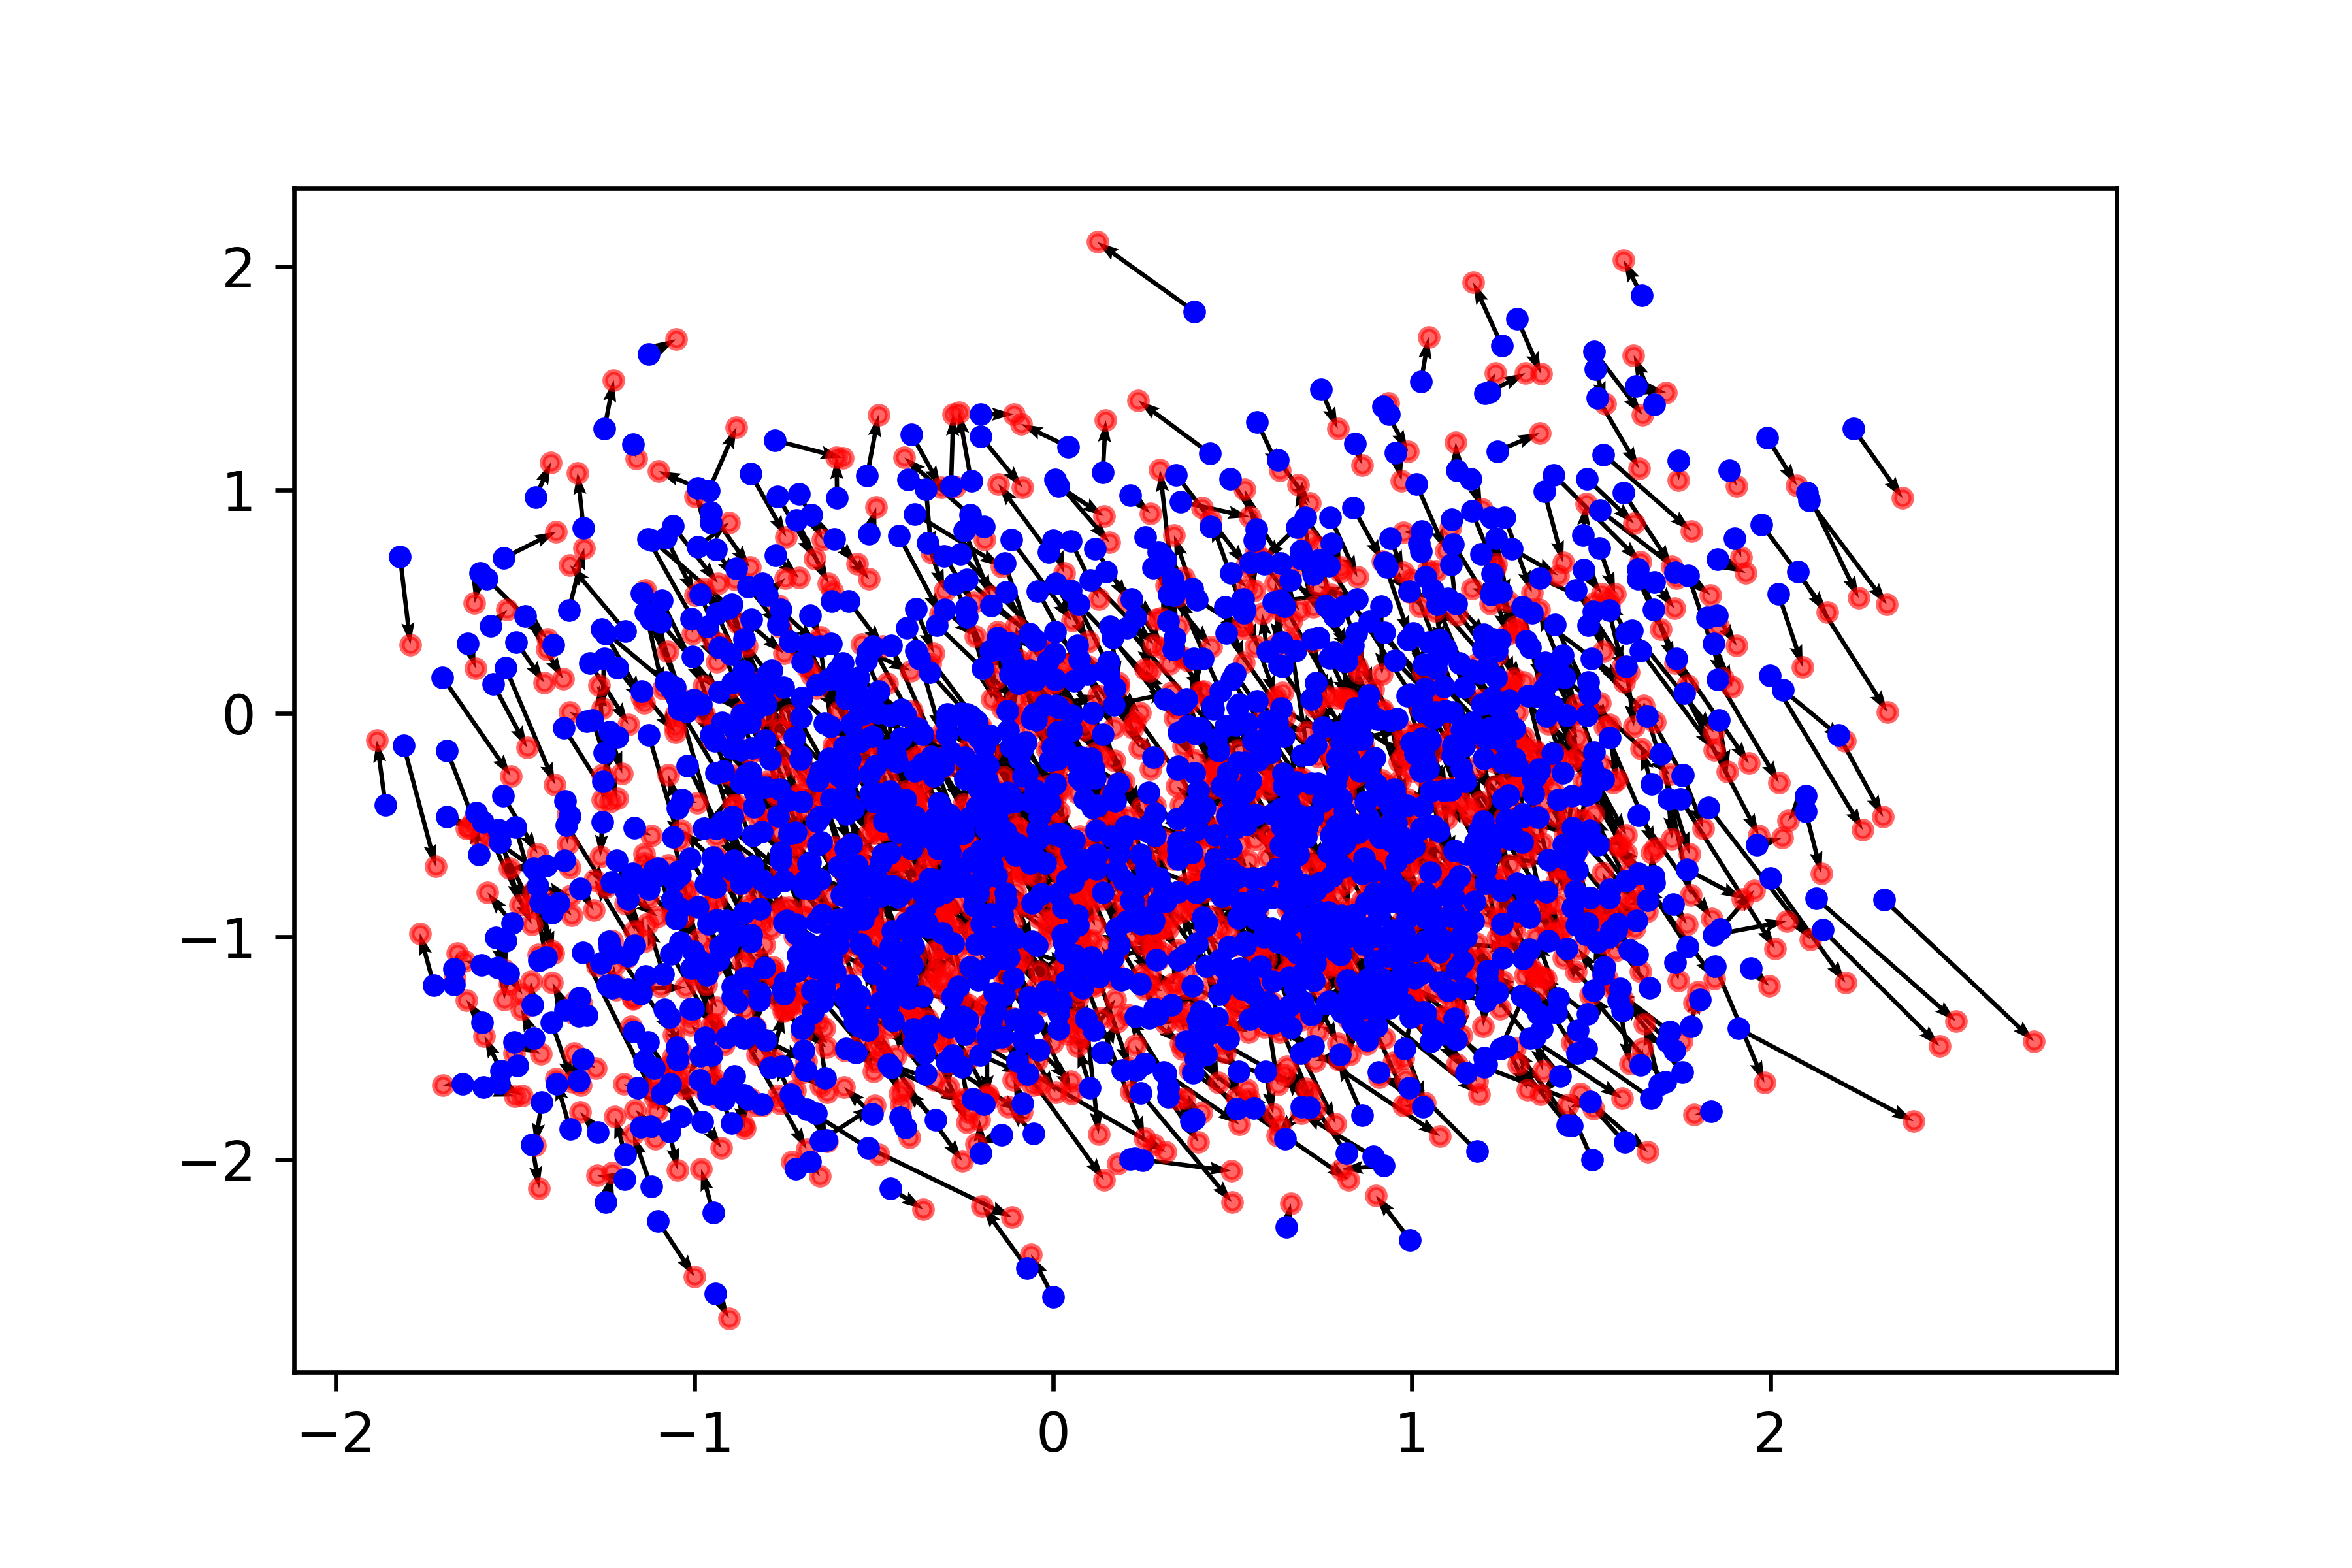
\includegraphics[width=\linewidth]{latentspace_species.png} 
%    \vspace{4ex}
%  \end{minipage}%%
%  \begin{minipage}[b]{0.5\linewidth}
%    \centering
%    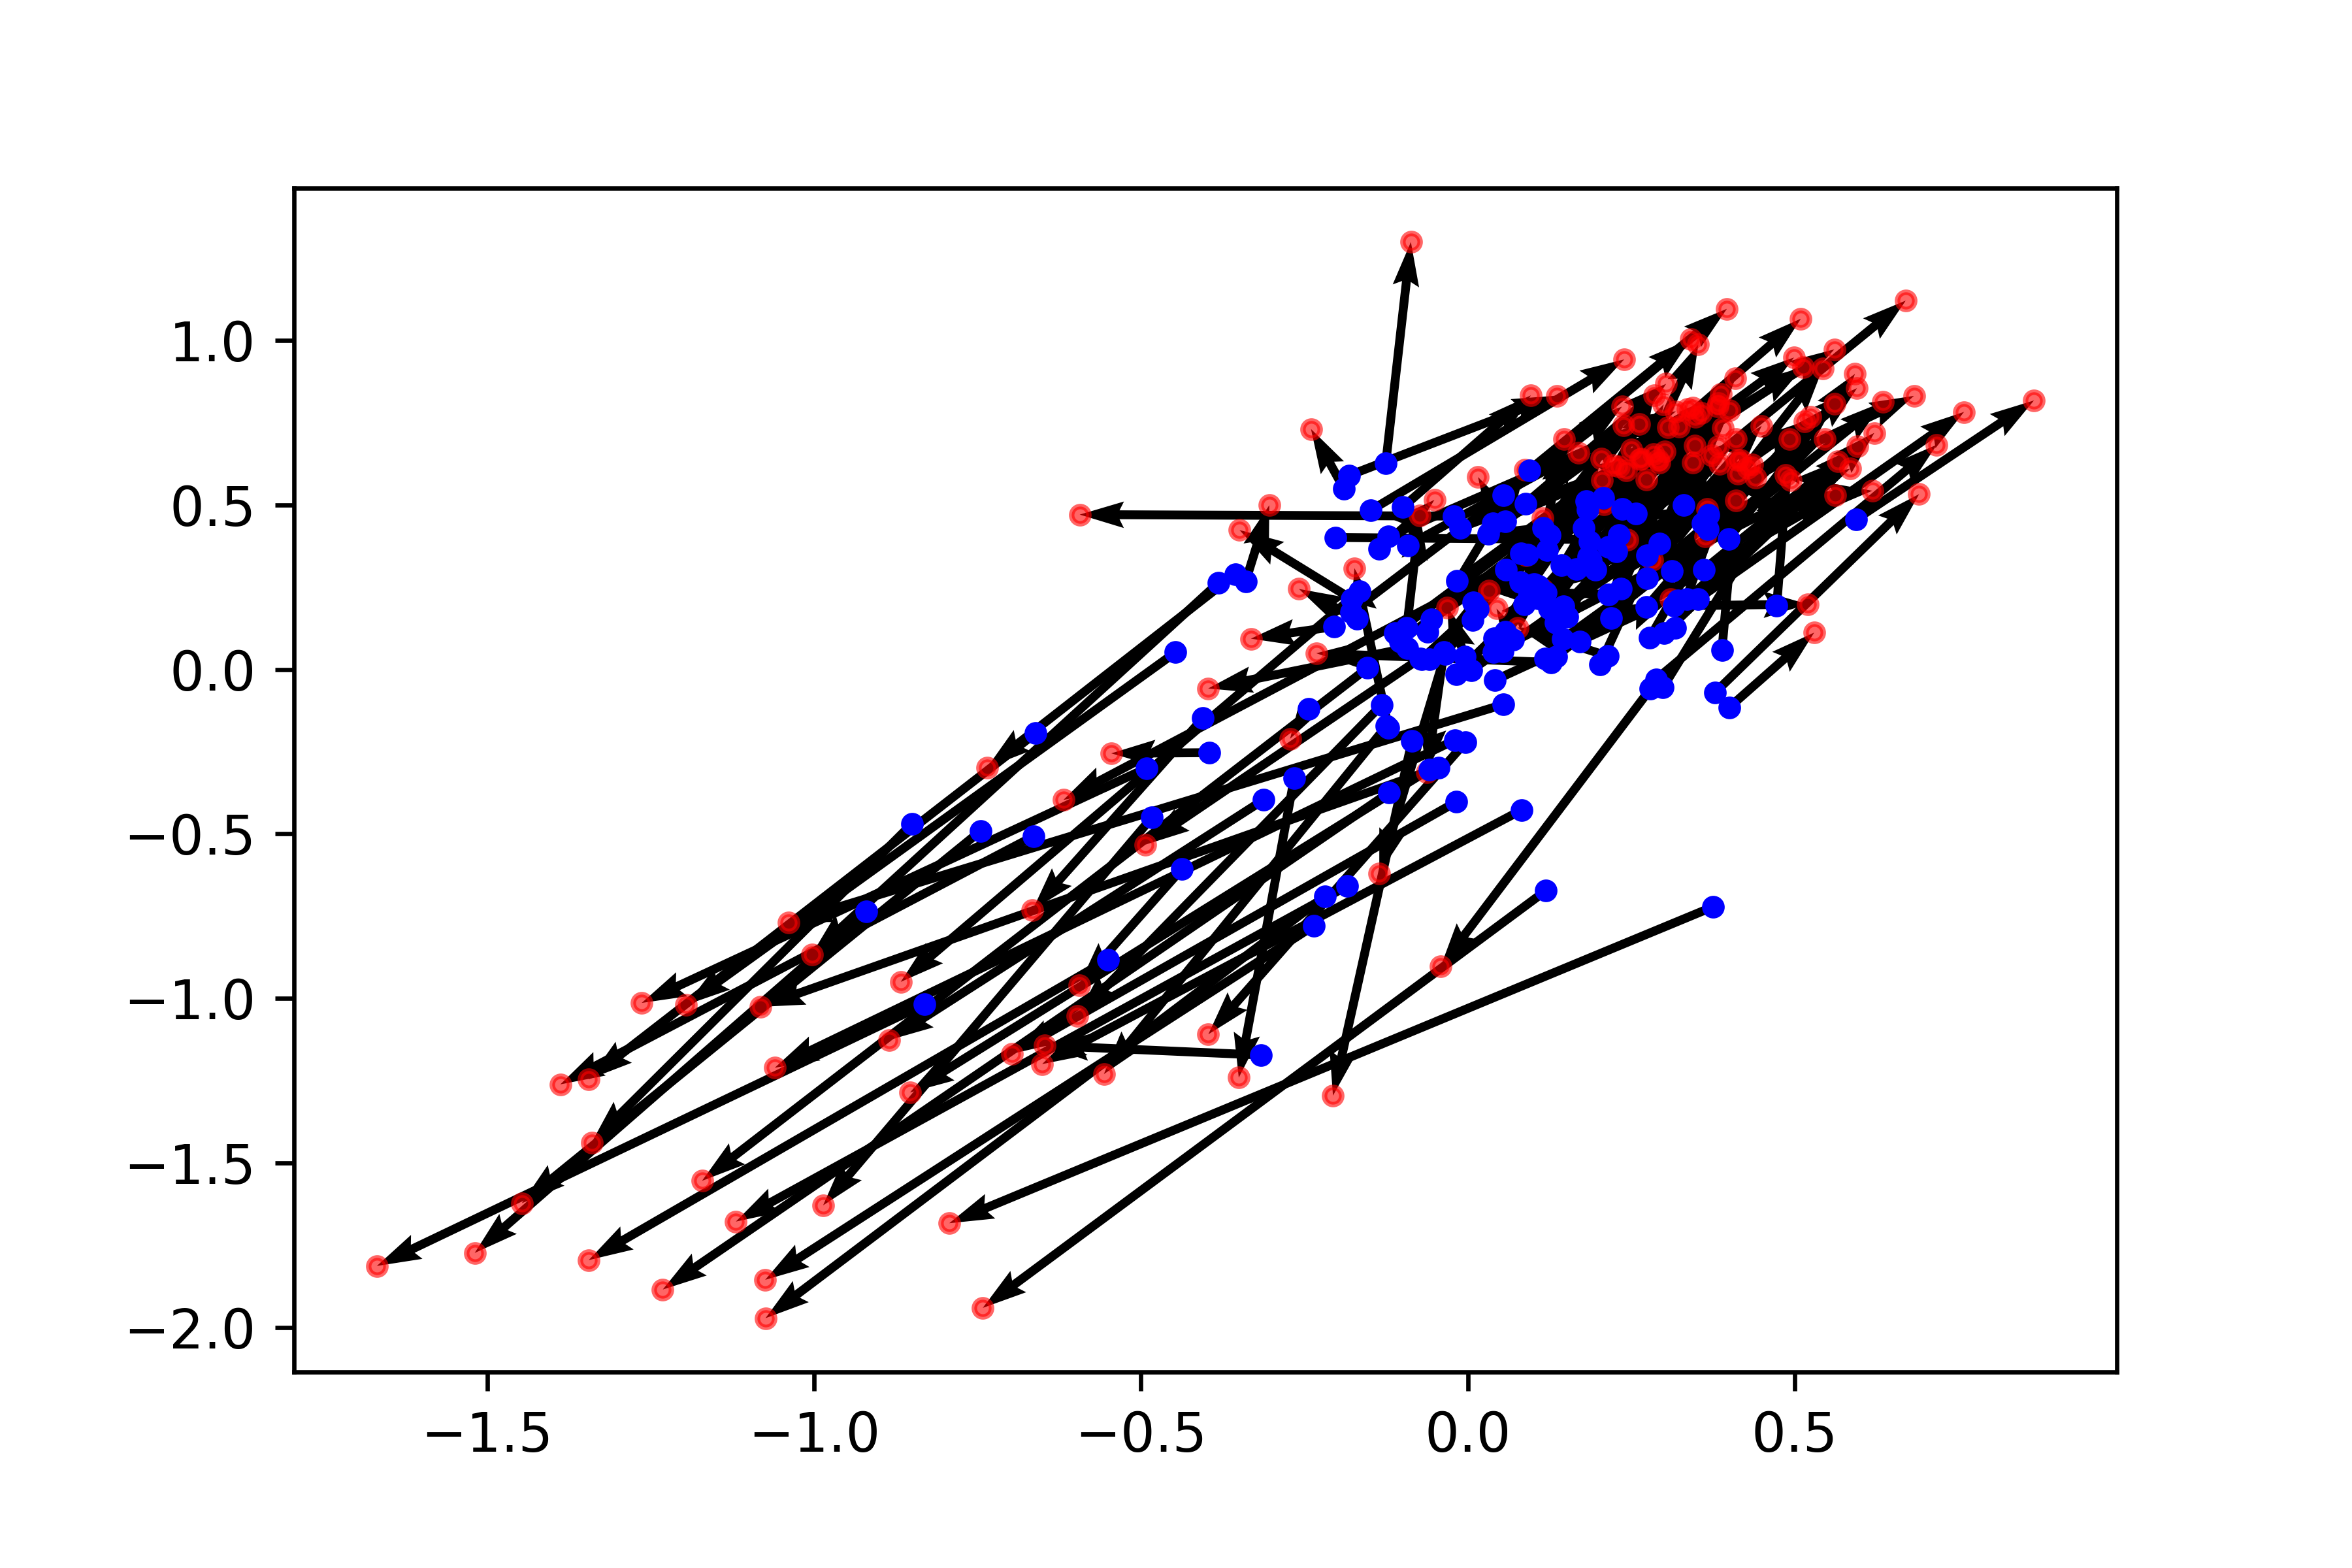
\includegraphics[width=\linewidth]{latentspace_region.png} 
%    \vspace{4ex}
%  \end{minipage}  
%\caption{Latent space initial and final configurations. The black arrows shows the movement in space from the initial state (blue) to the final state (red).}
%\label{fig:latentspace_config}
%\end{figure}
%\end{frame}


\begin{frame}
\begin{figure}[H] 
  \label{ fig7} 
  \begin{minipage}[b]{0.5\linewidth}
    \centering
    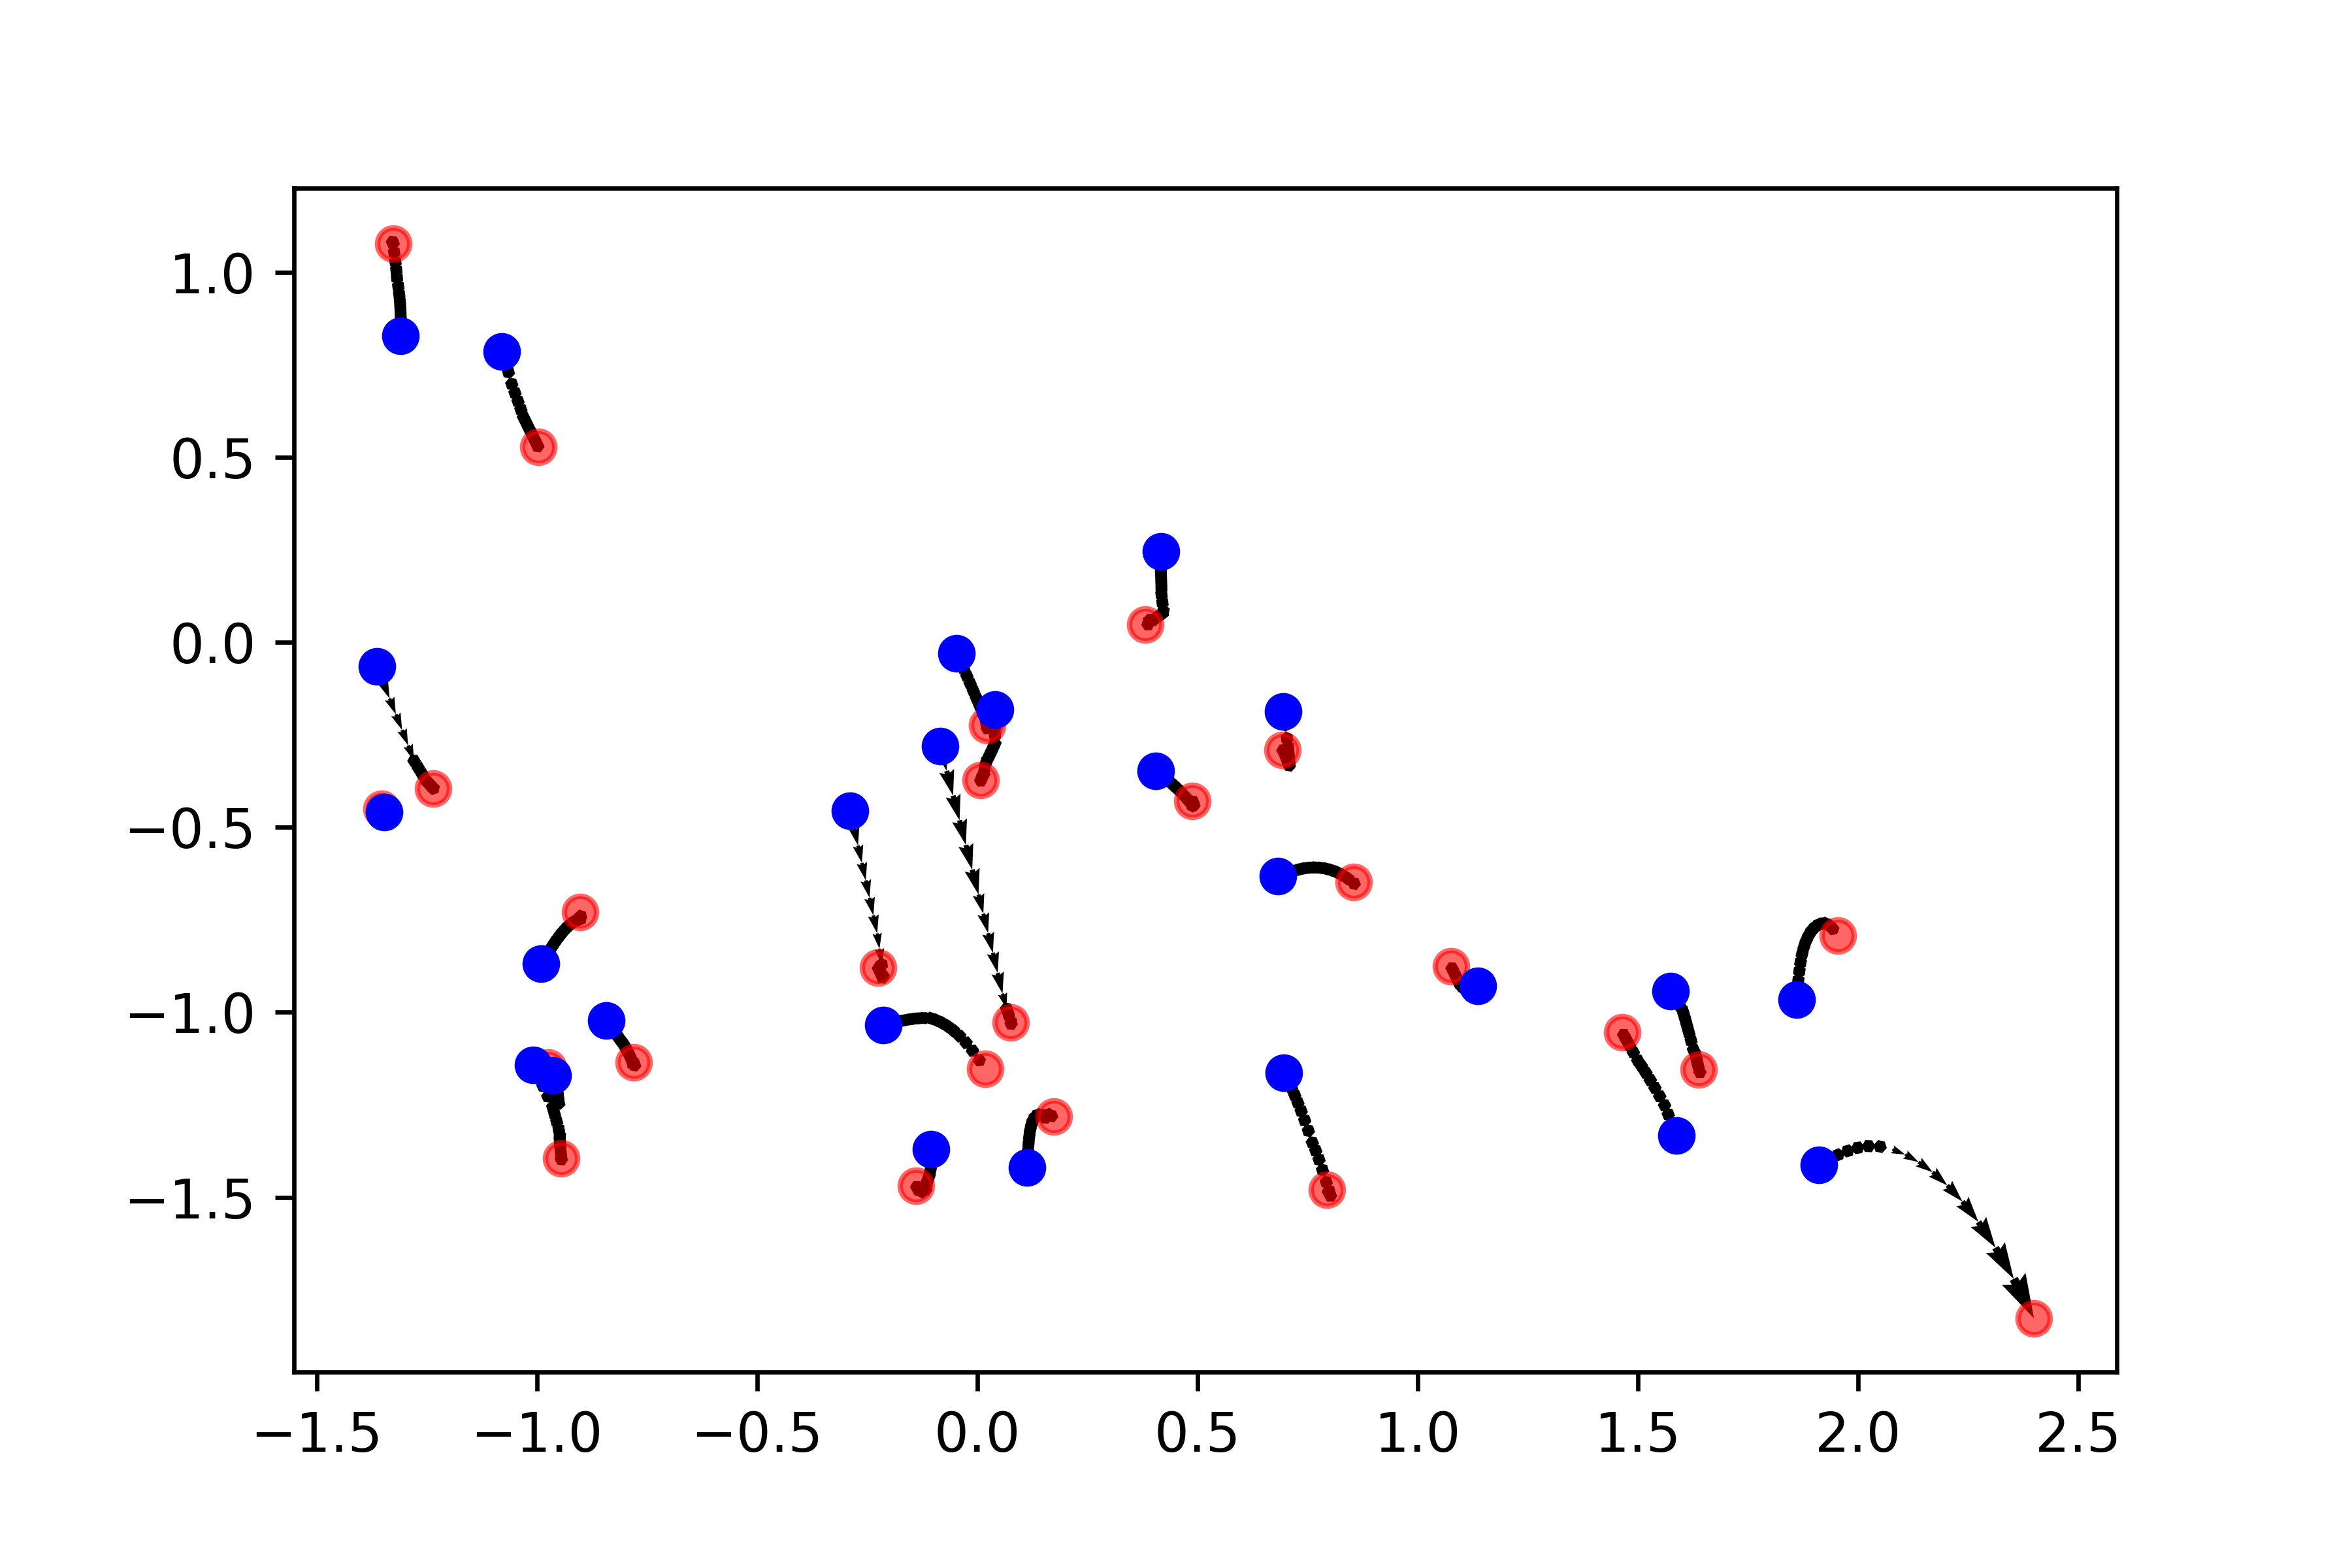
\includegraphics[width=\linewidth]{latentspace_afew_species.png} 
    \vspace{4ex}
  \end{minipage}%%
  \begin{minipage}[b]{0.5\linewidth}
    \centering
    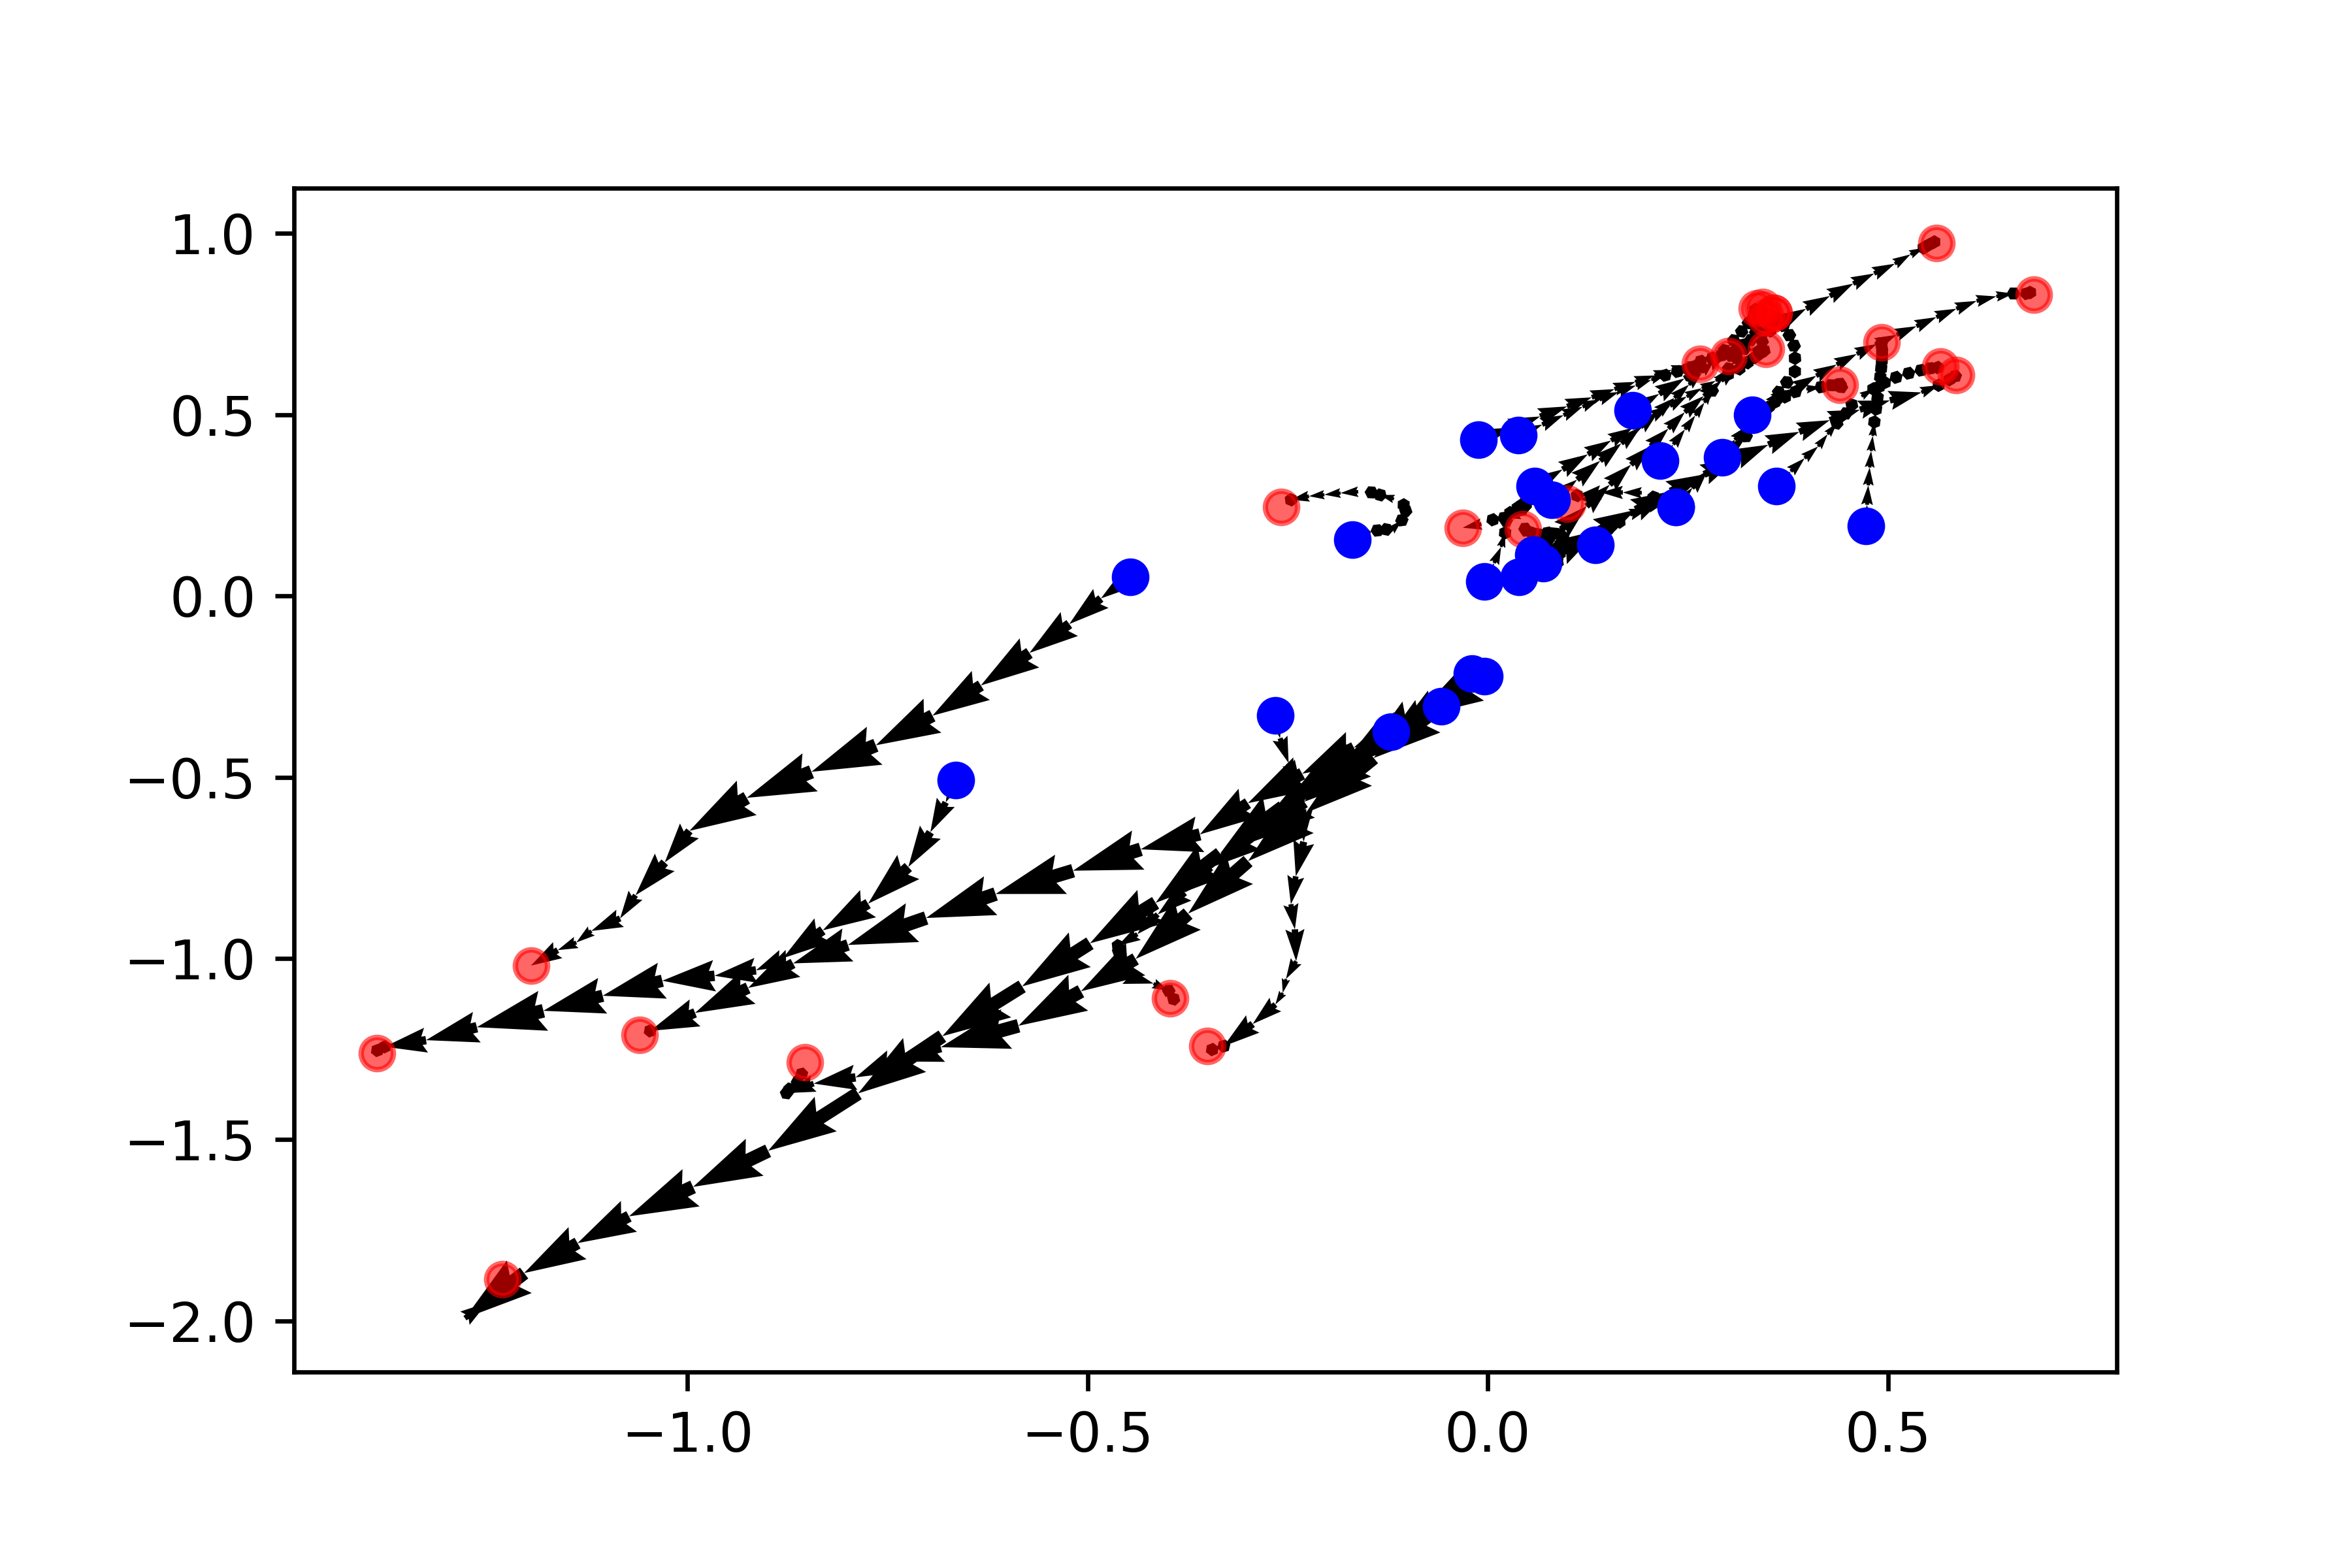
\includegraphics[width=\linewidth]{latentspace_afew_region.png} 
    \vspace{4ex}
  \end{minipage}  
\caption{A set of 25 randomly chosen species (left) and regions (right) and their dynamics in the latent space.}
\label{fig:latentspace_afew}
\end{figure}
\end{frame}


\begin{frame}
Species that move in a similar way inside the latent space tend to co-invade. Similarly, regions that move analogously will have the tendency to be co-invaded by the same group of species.

\bigskip 

Applying \textit{Ordering points to identify the clustering structure} OPTICS to the species and regions in the latent space detected 67 clusters for species and 5 clusters for regions.

\end{frame}

\begin{frame}

\begin{figure}[H] 
  \begin{minipage}[b]{0.5\linewidth}
    \centering
    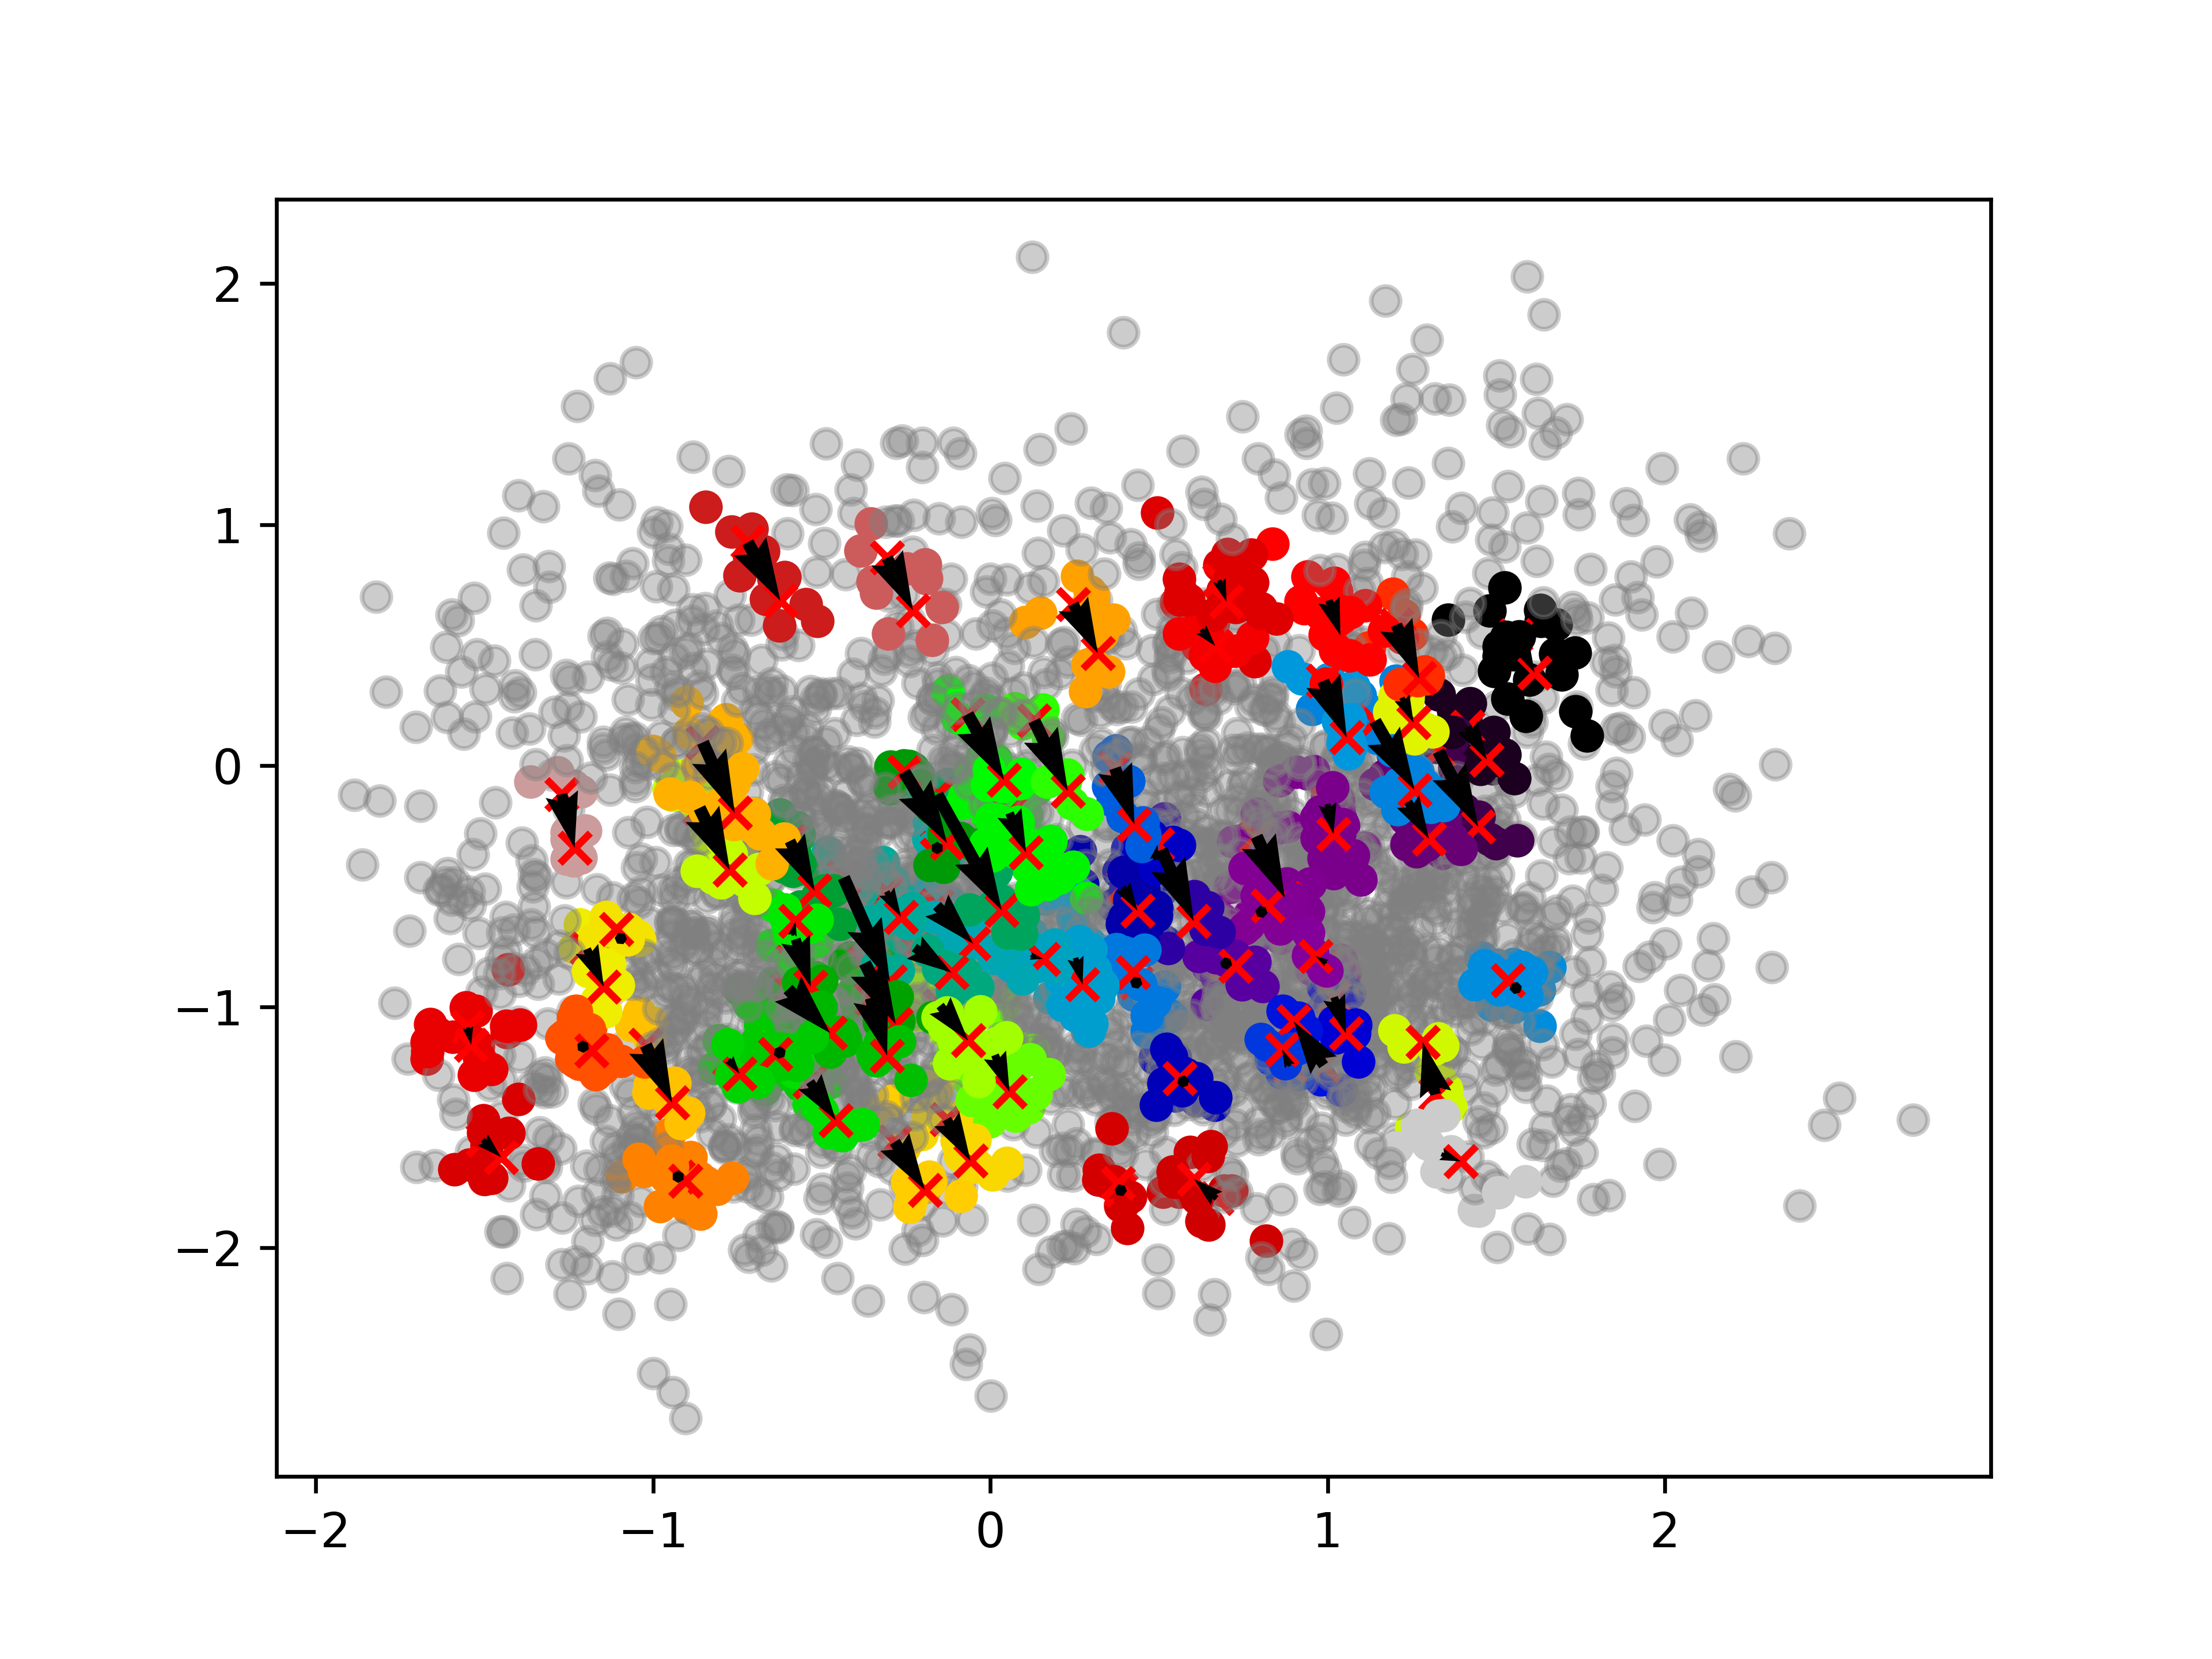
\includegraphics[width=\textwidth]{latentspace_cluster_species.png}
    \vspace{4ex}
  \end{minipage}%%
  \begin{minipage}[b]{0.5\linewidth}
    \centering
    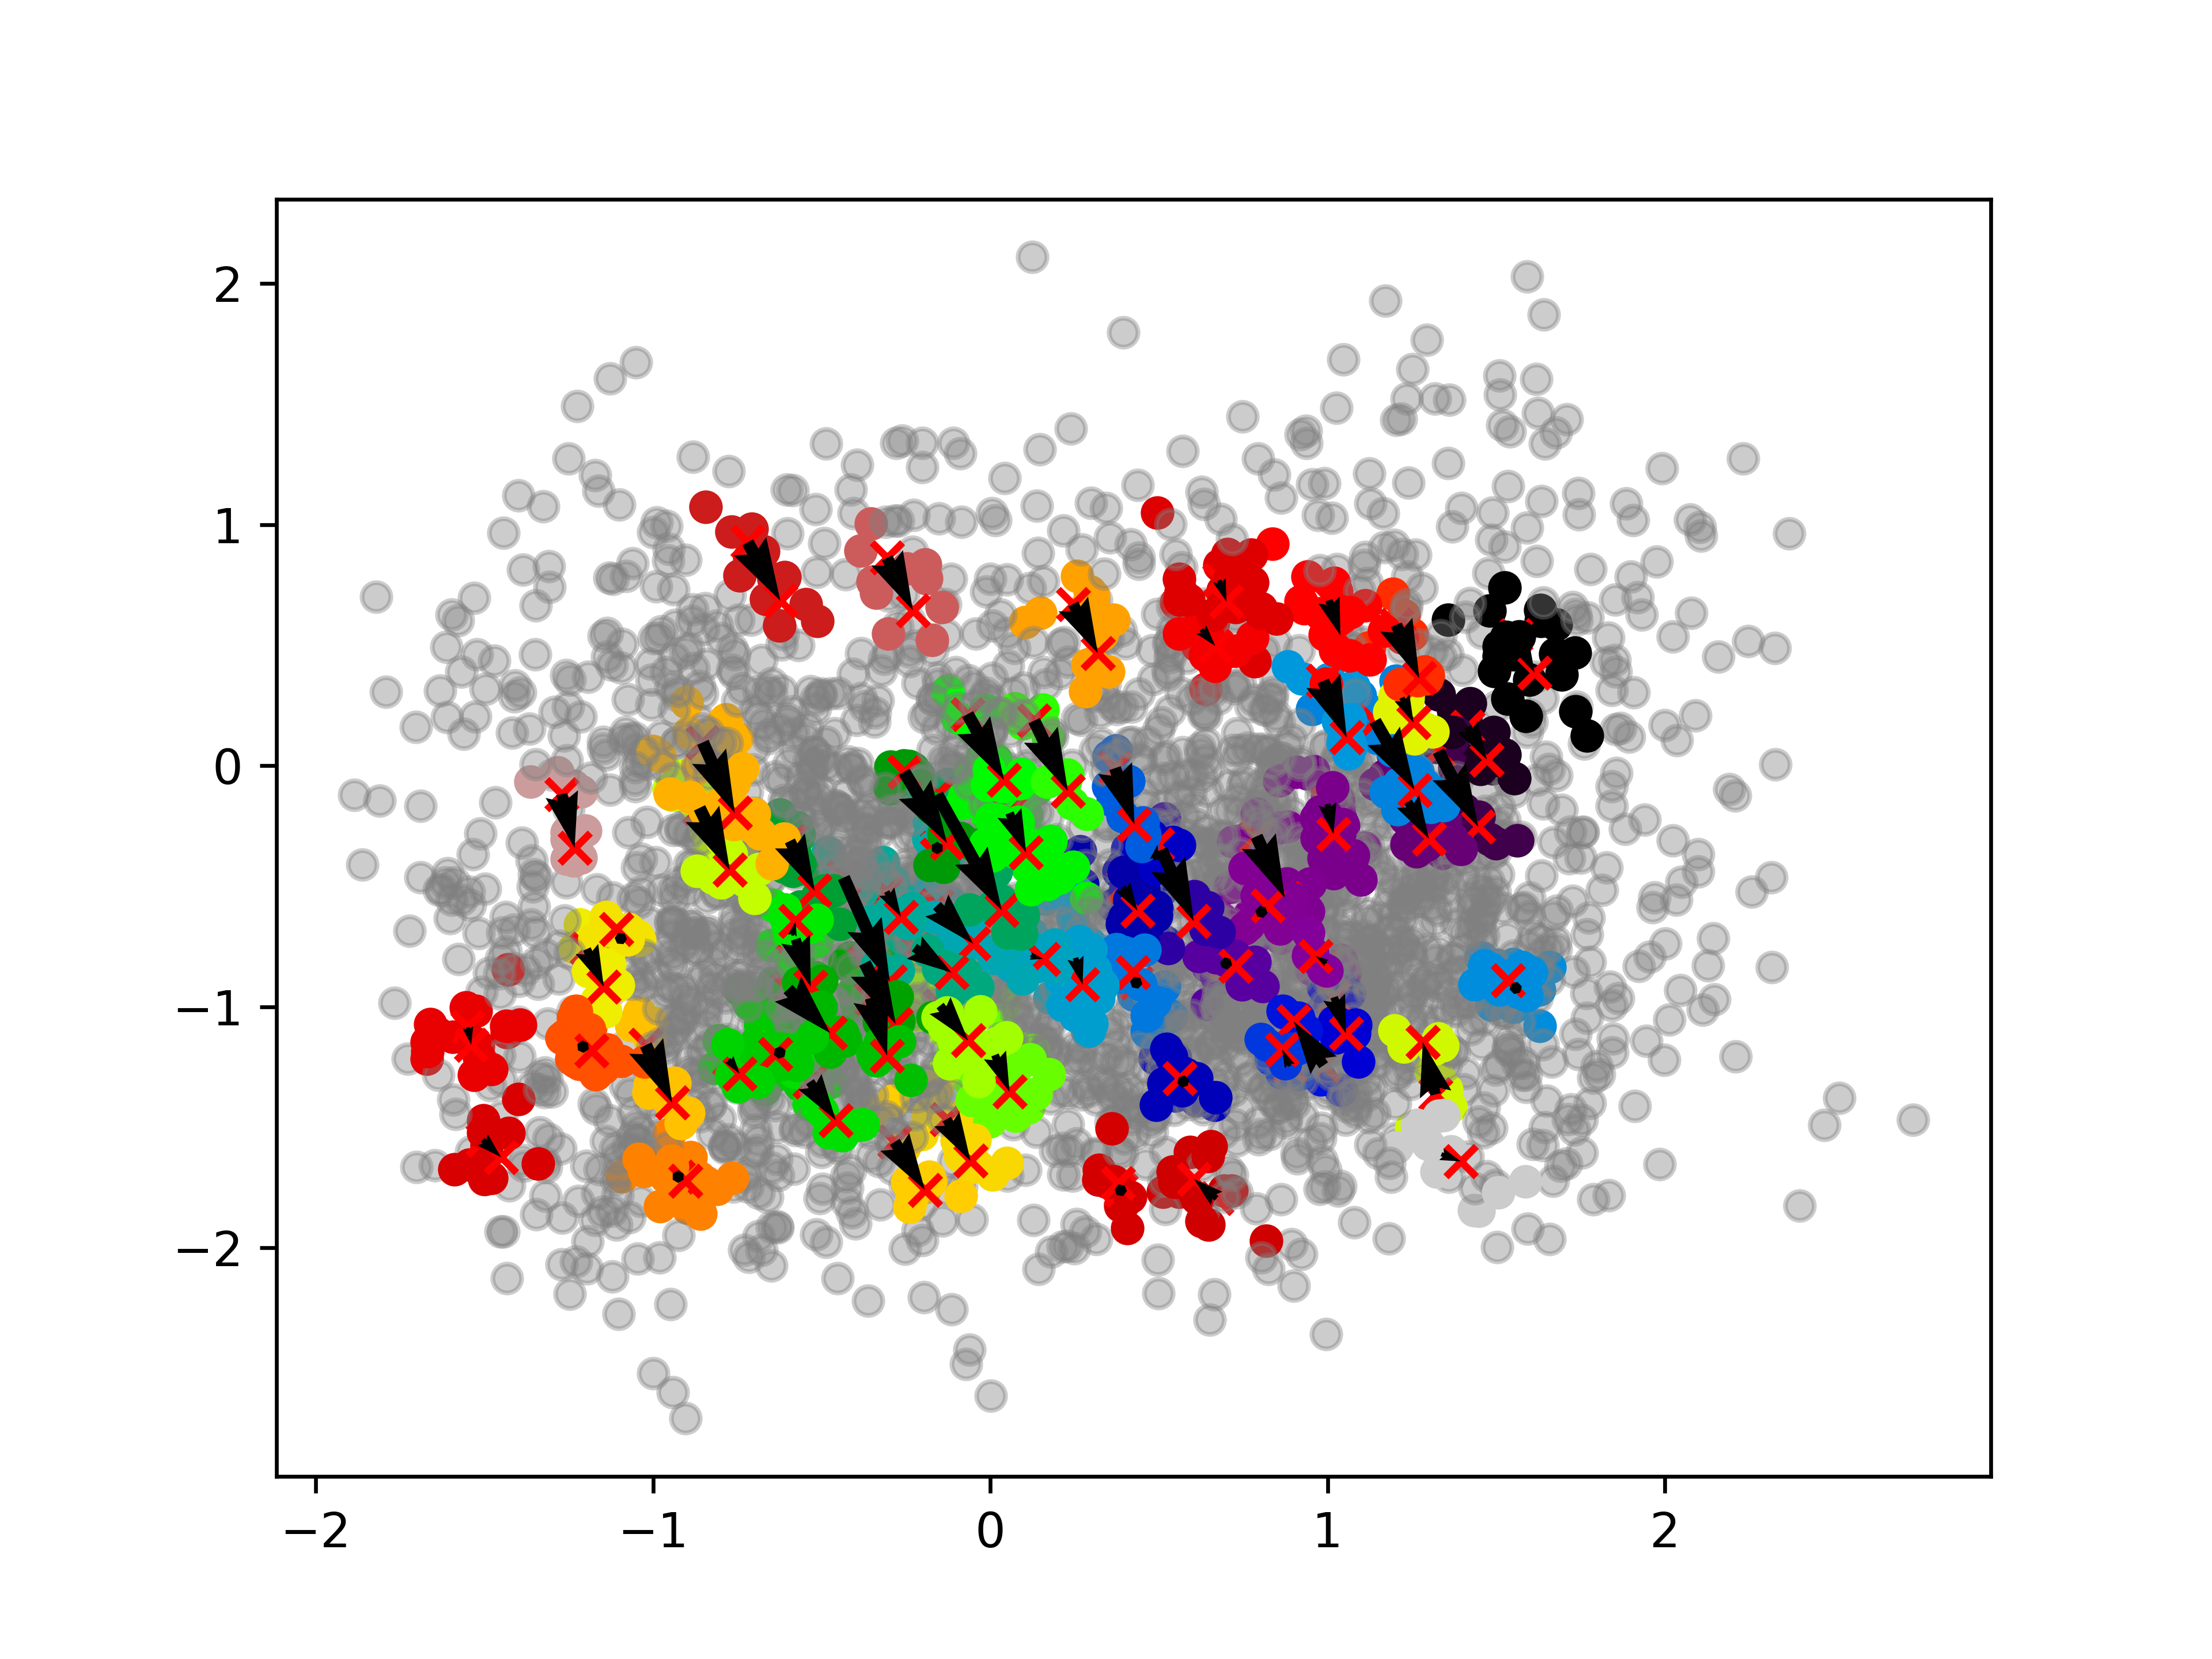
\includegraphics[width=\textwidth]{latentspace_cluster_region.png}
    \vspace{4ex}
  \end{minipage}  
\caption{Latent space initial and final configurations. The black arrows shows the movement in space from the initial state to the final state.}
\label{fig:latentspace_cluster}
\end{figure}
\end{frame}

%----------------------------------------------------------------------------------------
%	DISCUSSION
%----------------------------------------------------------------------------------------

%\begin{frame}
%
%\begin{figure}[H] 
%  \label{ fig7} 
%  \begin{minipage}[b]{0.5\linewidth}
%    \centering
%        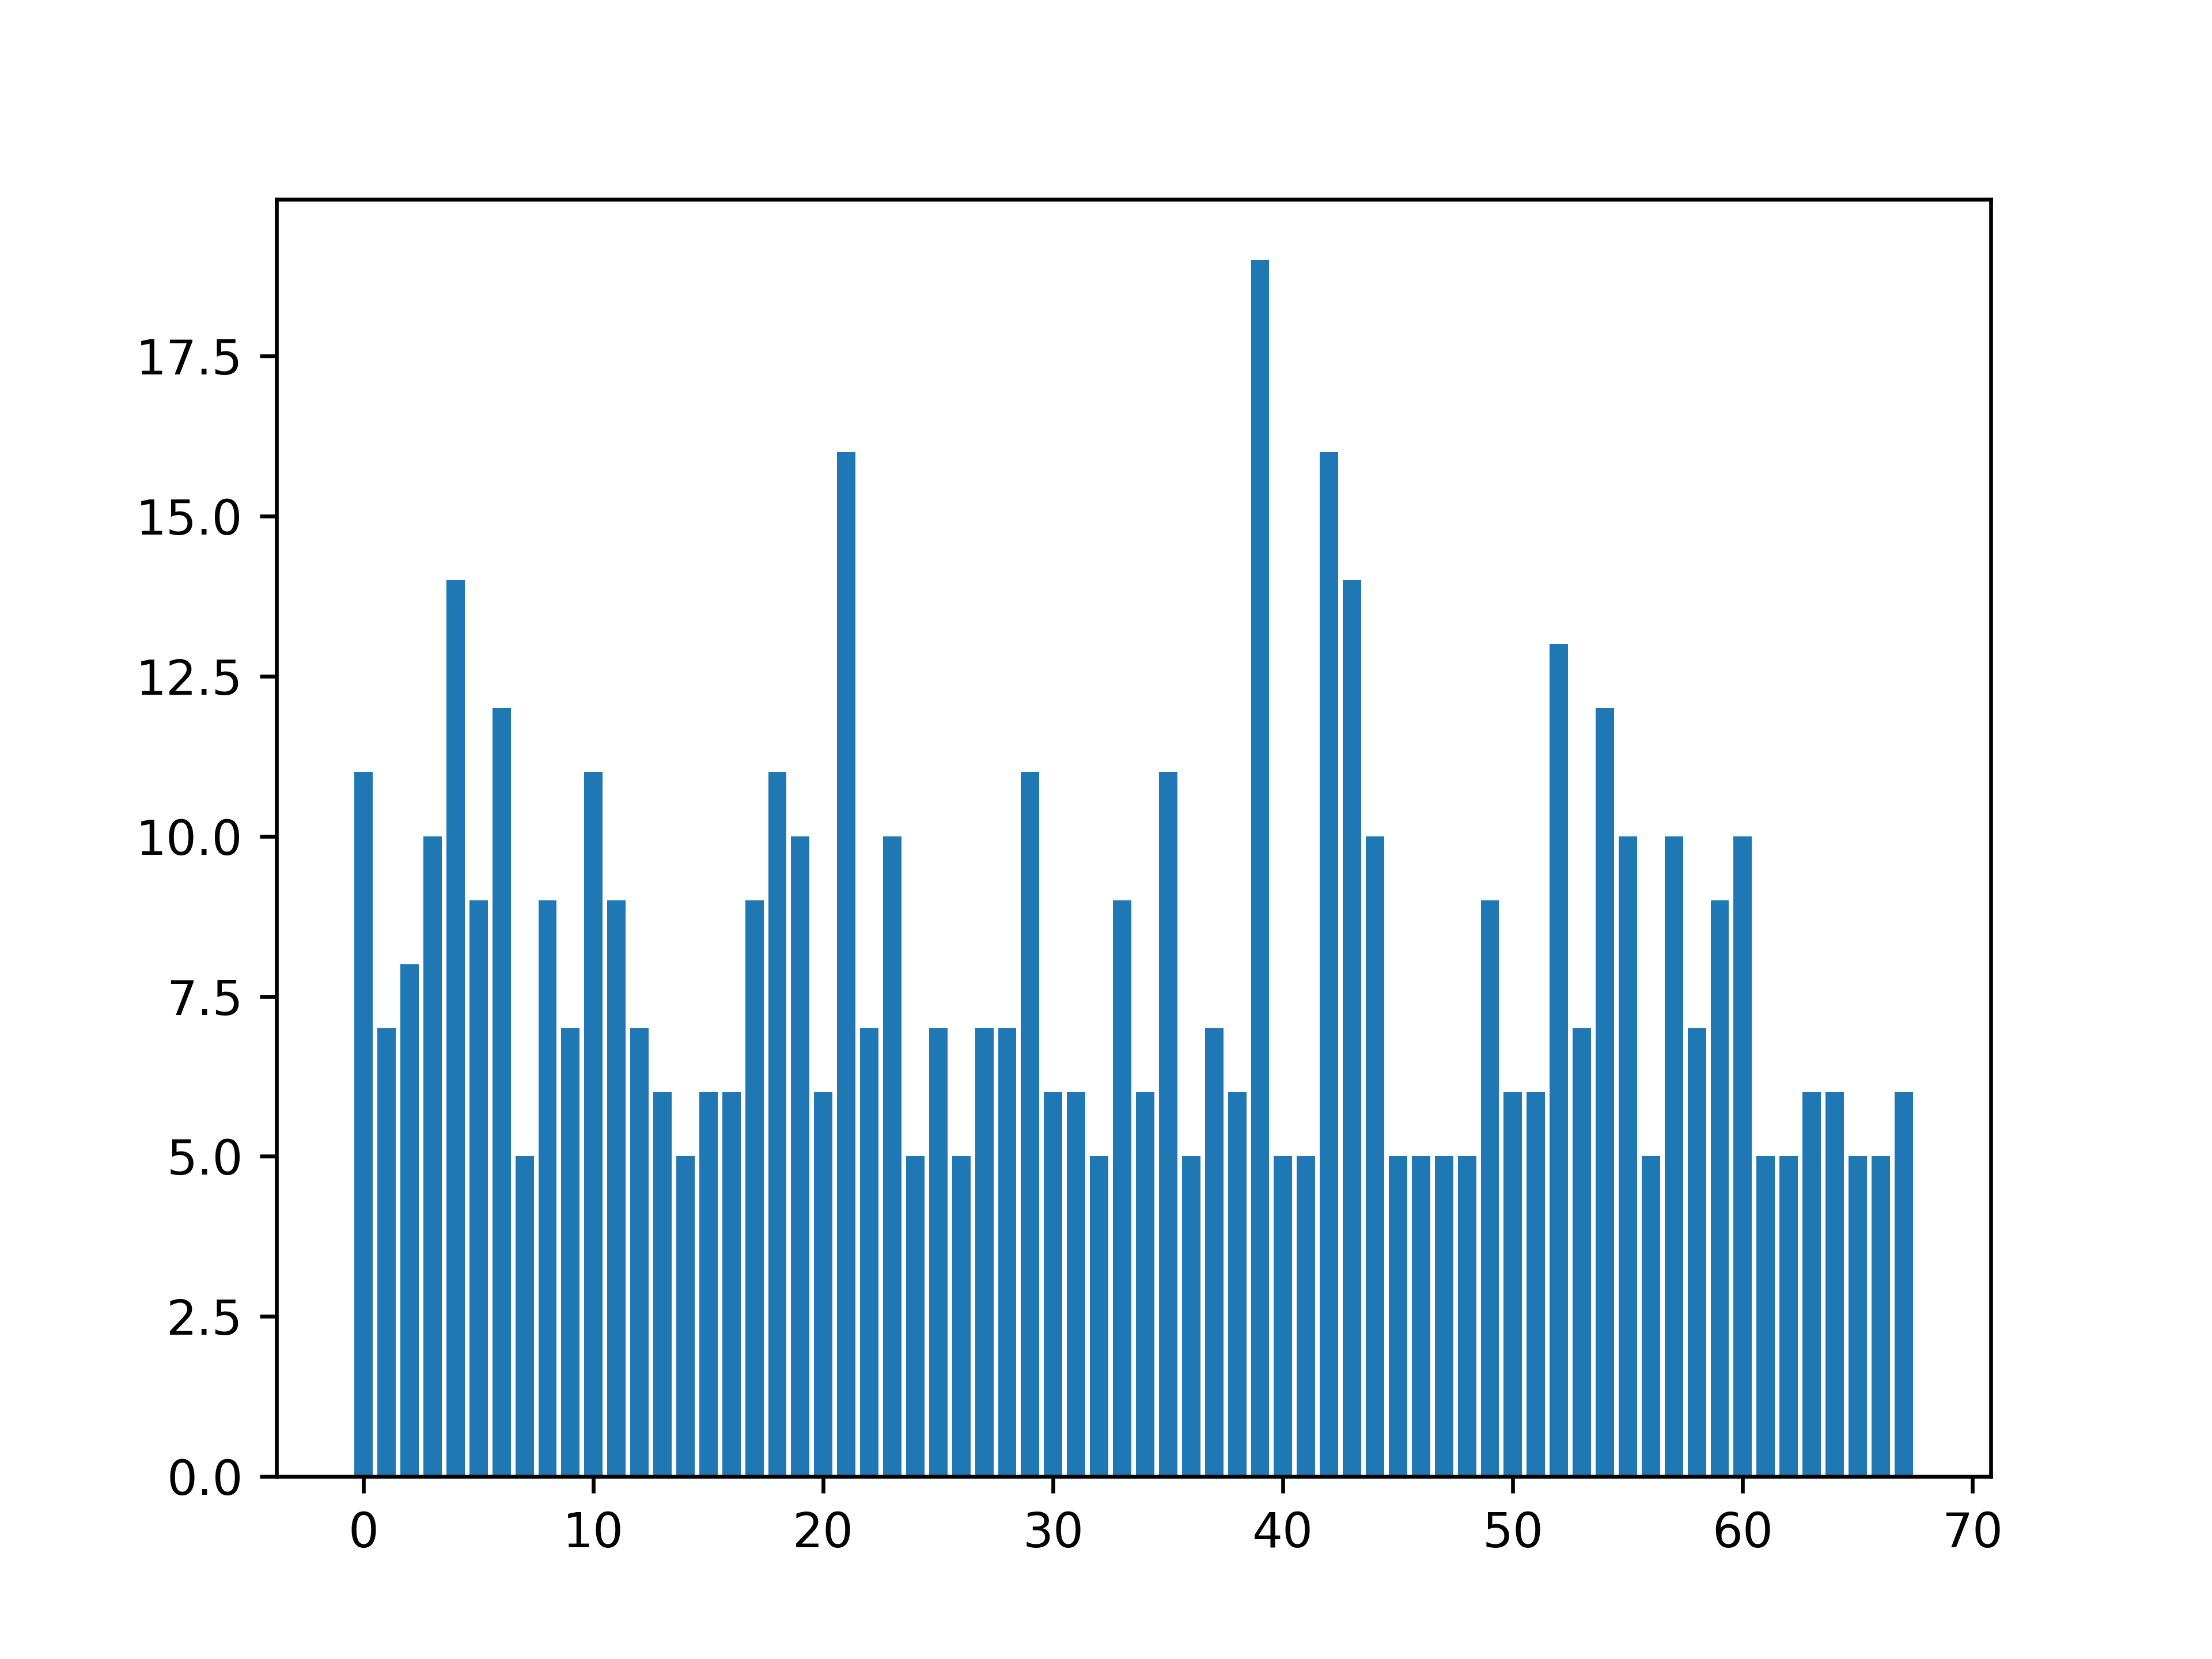
\includegraphics[width=0.75\textwidth]{cluster_distribution_species.png}
%%    \caption{Size distribution of the \\ cluster of species.}
%    \vspace{4ex}
%  \end{minipage}%%
%  \begin{minipage}[b]{0.5\linewidth}
%    \centering
%     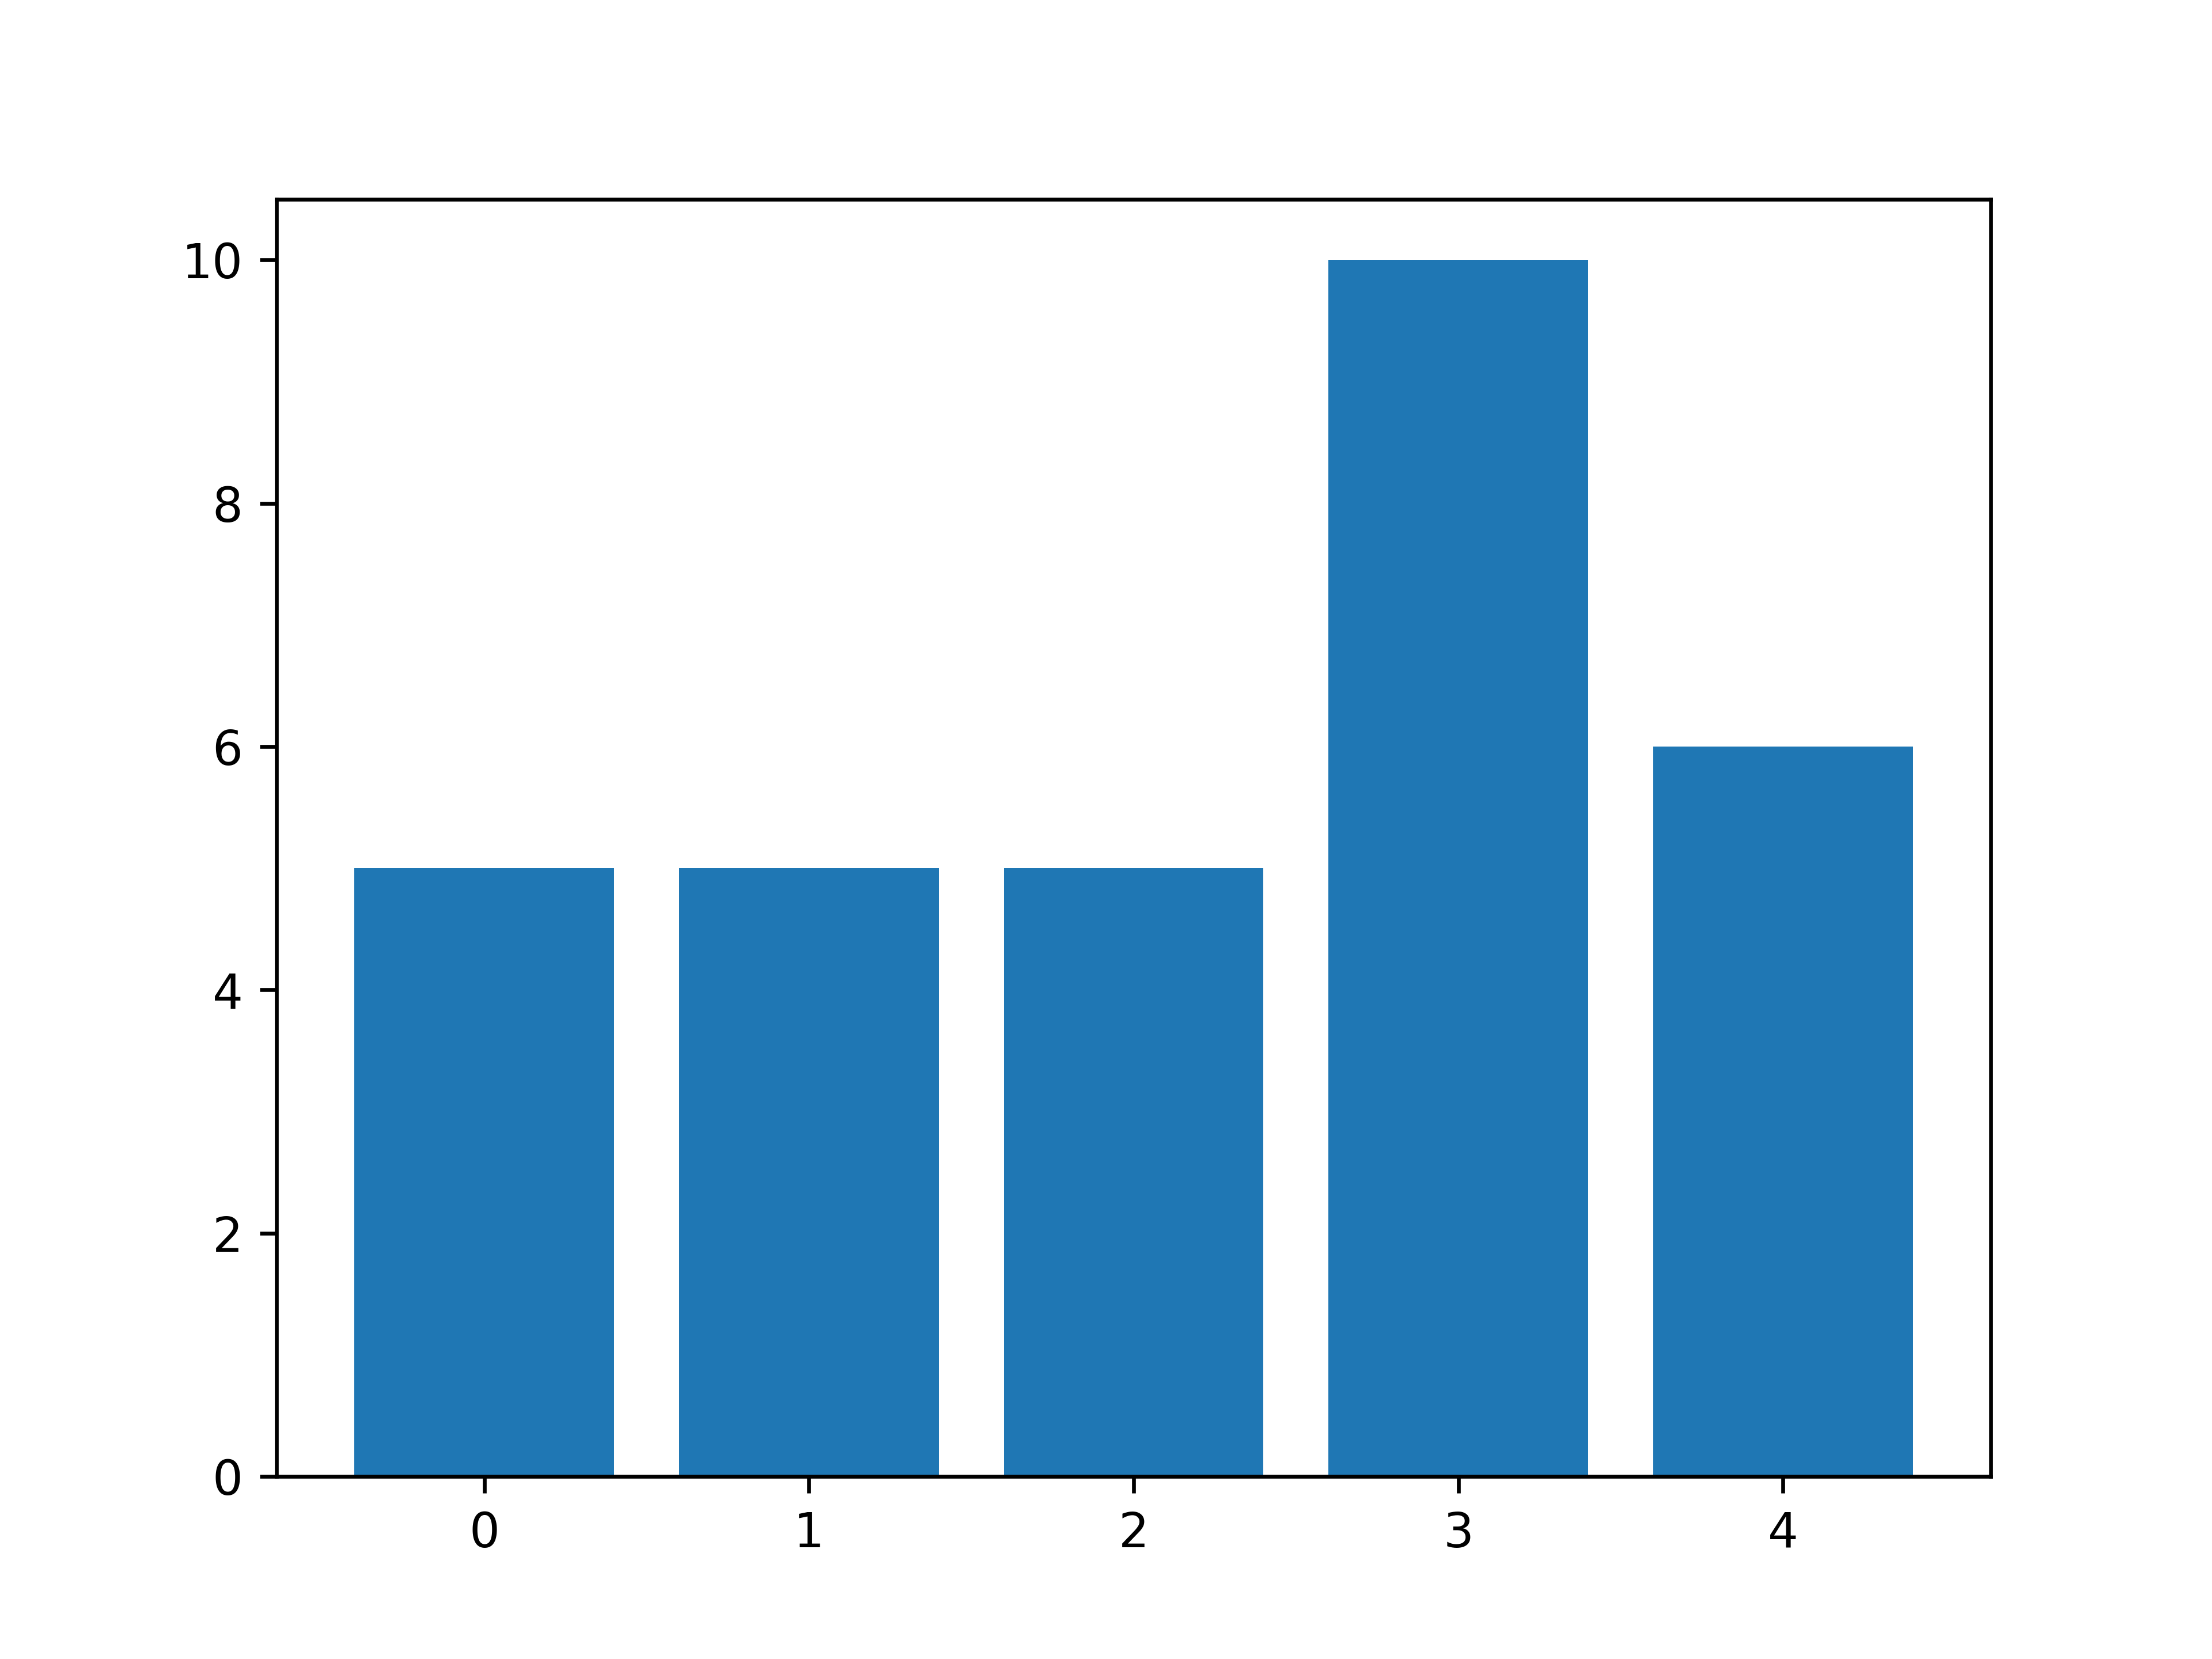
\includegraphics[width=0.75\textwidth]{cluster_distribution_region.png}
%%    \caption{Size distribution of the \\ cluster of region.}
%    \vspace{4ex}
%  \end{minipage} 
%%\caption{Cluster dimension.}
%\caption{Size distribution of the cluster of species (left) and region (right).}
%\label{fig:cluster_density}
%\end{figure}
%\end{frame}

\begin{frame}
%TODO table is outside....
\frametitle{Insights from the species clusters}
We select the five largest species and clusters.
\begin{table}[H]
\smaller
\centering
\begin{tabular}{|l|l|l|l|l|l|}
\hline
             & Cluster 0 & Cluster 1         & Cluster 2  & Cluster 3           & Cluster 4 \\ \hline
Algae           &           &            & 11 \%      &            &            \\ \hline
Birds           & 7 \%      & 6 \%       &            &            & 7 \%       \\ \hline
Crustaceans     & 7 \%      &            & 16 \%      & 6 \%       &            \\ \hline
Fishes          &           &            & 5 \%       & 6 \%       &            \\ \hline
Fungi           &           &            &            & 6 \%       &            \\ \hline
Insects         & 14 \%     & 12 \%      & 16 \%      &            & 36 \%      \\ \hline
Mammals         & 7 \%      &            &            &            &            \\ \hline
Reptiles        &           & 6 \%       &            &            &            \\ \hline
Vascular plants & 64 \%     & 75 \%      & 53 \%      & 81 \%      & 57 \%      \\ \hline
\end{tabular}
\caption{Species clusters composition.}
\label{table:clusters_species}
\end{table}

\end{frame}

\begin{frame}
\frametitle{Insights from the reguon clusters}
We select the five largest species and clusters.

\begin{table}[H]
\smaller
\centering
\begin{tabular}{|l|l|l|l|l|}
\hline
Cluster 0 & Cluster 1                 & Cluster 2  & Cluster 3           & Cluster 4                \\ \hline
Russia    & Armenia                   & Lesotho    & Peru                & Iraq                     \\ \hline
Italy     & Chad                      & Mauritania & Andorra             & Nicaragua                \\ \hline
Canada    & Iran  & Gibraltar  & Belize              & Niger                    \\ \hline
Estonia   & Mongolia                  & Nepal      & Burkina Faso        & Vietnam                  \\ \hline
Slovakia  & Somalia                   & Suriname   & Libya               & Zambia                   \\ \hline
          &                           &            & Palestine & CAR \\ \hline
          &                           &            & Senegal             &                          \\ \hline
          &                           &            & Tajikistan          &                          \\ \hline
          &                           &            & Gabon               &                          \\ \hline
          &                           &            & Congo               &                          \\ \hline
\end{tabular}
\caption{Region clusters composition.}
\label{table:clusters_region}
\end{table}

\end{frame}

\begin{frame}
\begin{figure}[ht]
    \centering
    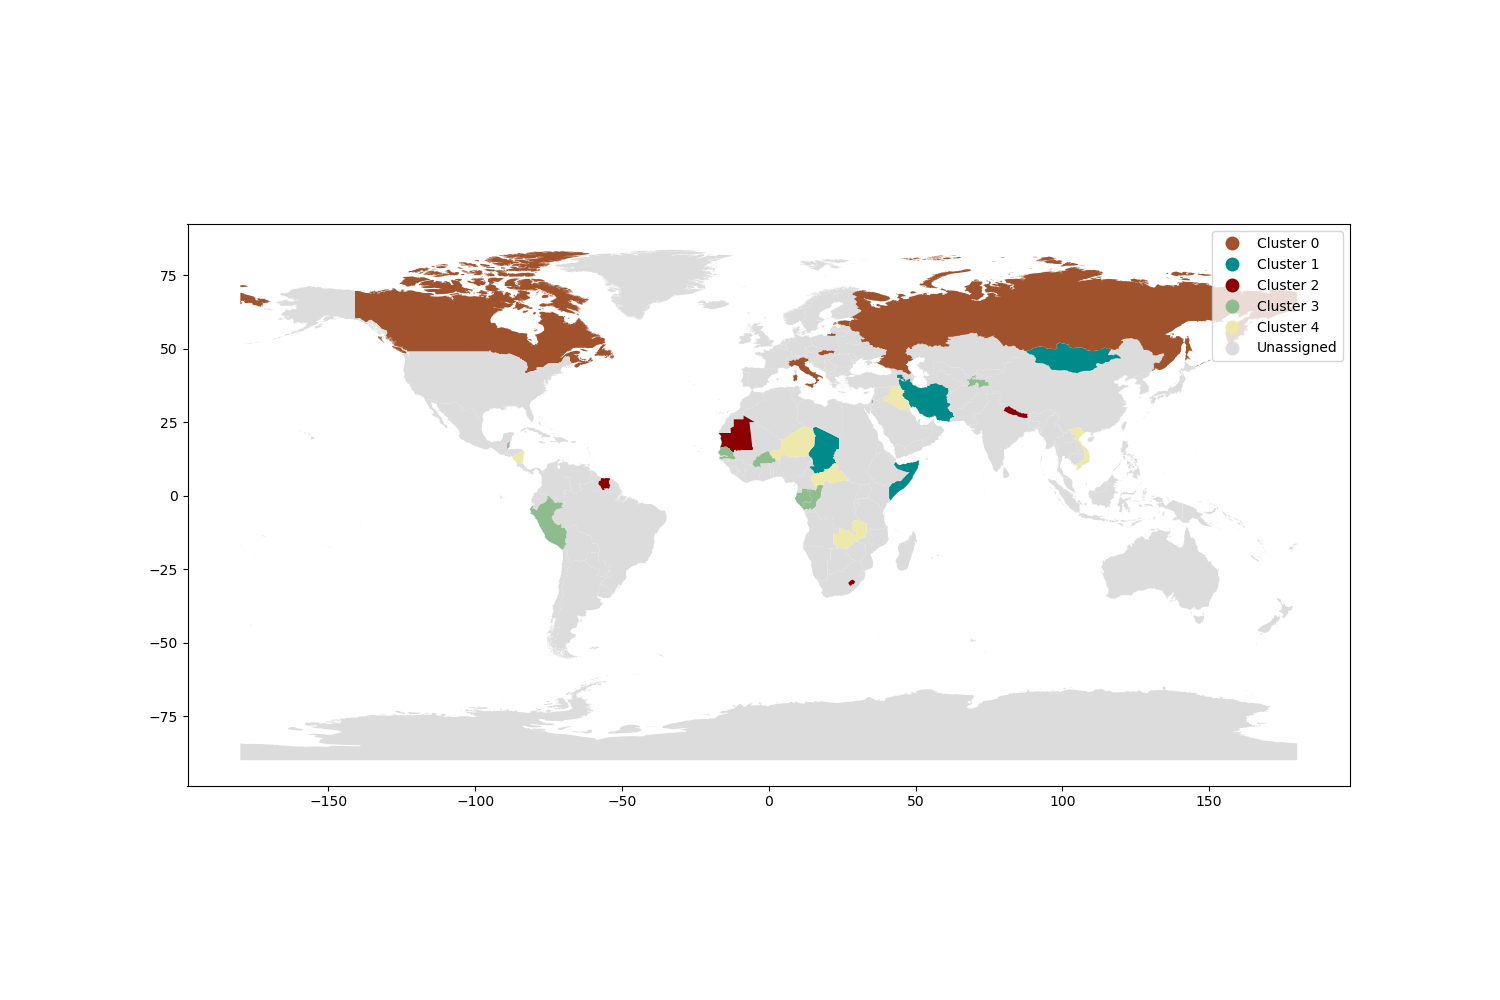
\includegraphics[width=0.85\textwidth]{region_geospatial_cluster.png}
    \caption{The five clusters of regions on the world map.}
    \label{fig:worldmap_cluster}
\end{figure}
\end{frame}

%----------------------------------------------------------------------------------------
%	Conclusion
%----------------------------------------------------------------------------------------

\section{Conclusion}

\begin{frame}
\frametitle{On the biasness of the dataset}


The First Records Dataset is currently the largest dataset available for first-time records of alien species, however:

\begin{itemize}
\item it is  an unevenly populated dataset towards taxonomic groups such as plants and insects
\item it is an unevenly populated dataset towards regions such as Europe as a whole
\item the information about the year of an alien species introduction in a region is not precise and most of the time does not correspond to the year of actual introduction, which might have happened decades later
\end{itemize}
\end{frame}

\begin{frame}
\begin{figure}[ht]
    \centering
    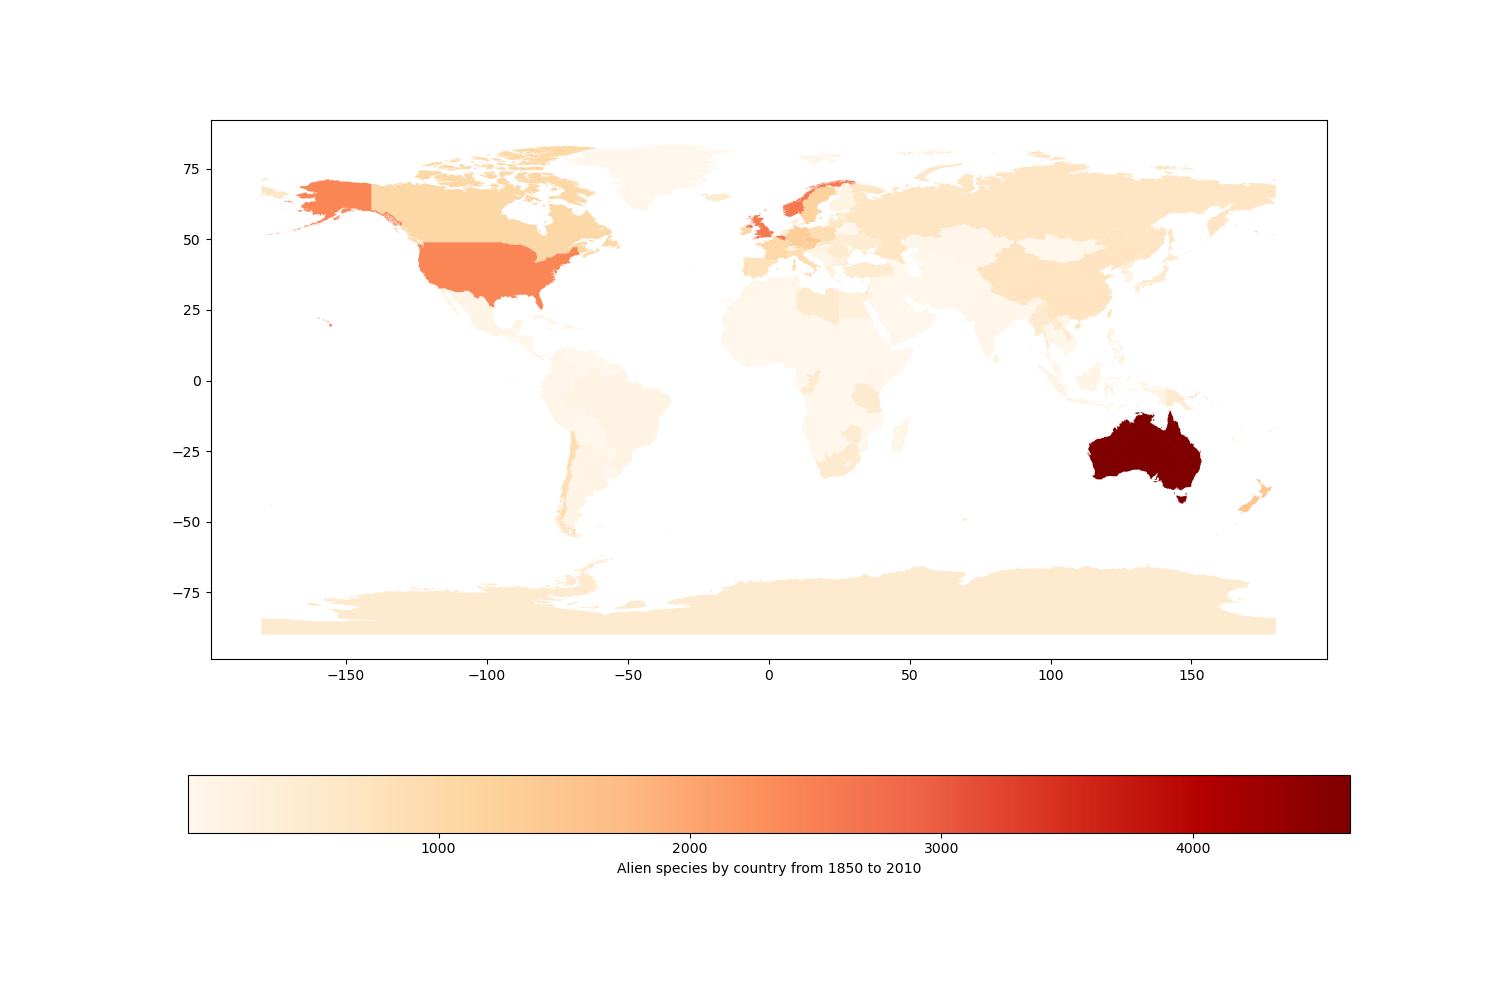
\includegraphics[width=0.85\textwidth]{region_invasion.png}
%    \caption{The five clusters of regions on the world map.}
%    \label{fig:worldmap_cluster}
\end{figure}
\end{frame}

%\begin{frame}
%\begin{figure}[ht]
%    \centering
%    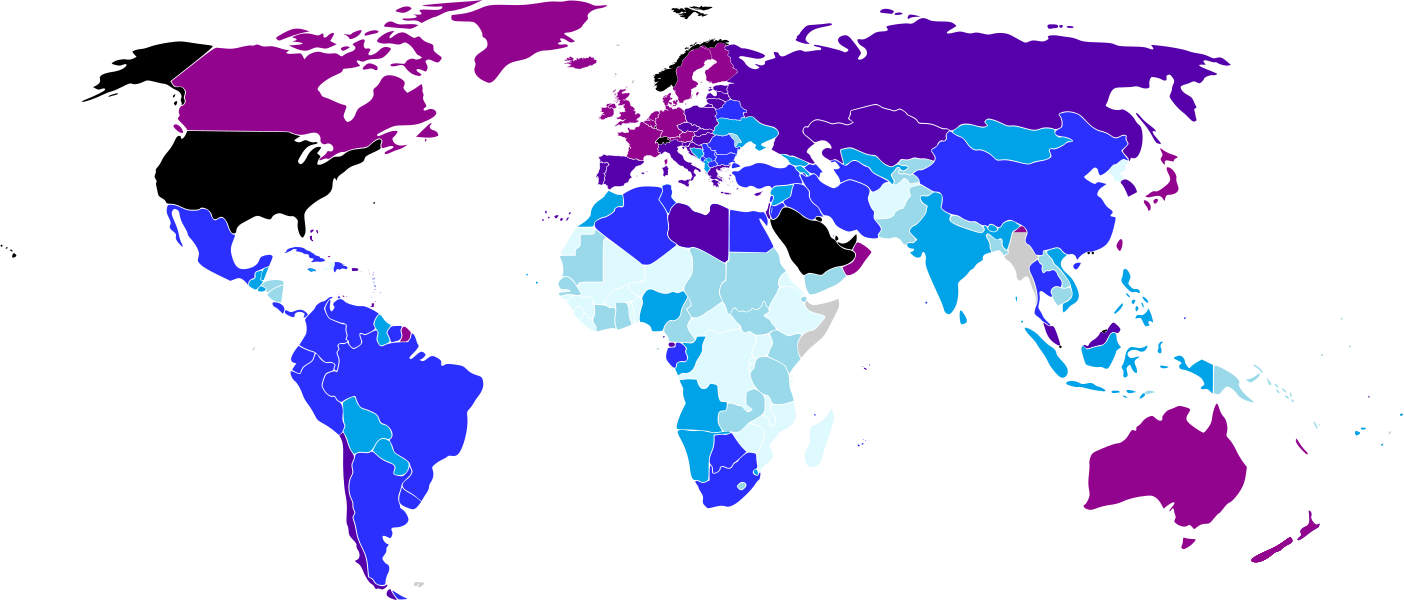
\includegraphics[width=0.85\textwidth]{region_gpd.png}
%%    \caption{The five clusters of regions on the world map.}
%    \label{fig:worldmap_cluster}
%\end{figure}
%\end{frame}


\begin{frame}
\frametitle{Conclusion}
%In this thesis:
\begin{itemize}
\item We proposed a relational event model with an underlying latent space formulation.
\item We showed a real world application of the model to the on-going problem of alien species.
\end{itemize}
\end{frame}

%Concluding, we showed how a relational event model can be applied to a bipartite dynamic network and extended by including a latent space configuration of the nodes. We then presented to the reader a framework to analyze the results based on a clustering algorithm. The improvements and extension of already existing tools such as relational event models into more advanced and efficient methods capable of performing time-dependent analysis such as the study of alien species' first records will help ecologists to investigate this ecological phenomenon in-depth and to come up with real-world actions. 


%\subsection{Columns}
%
%\begin{frame}
%	\frametitle{Multiple Columns}
%	\framesubtitle{Subtitle} % Optional subtitle
%	
%	\begin{columns}[c] % The "c" option specifies centered vertical alignment while the "t" option is used for top vertical alignment
%		\begin{column}{0.45\textwidth} % Left column width
%			\textbf{Heading}
%			\begin{enumerate}
%				\item Statement
%				\item Explanation
%				\item Example
%			\end{enumerate}
%		\end{column}
%		\begin{column}{0.5\textwidth} % Right column width
%			Lorem ipsum dolor sit amet, consectetur adipiscing elit. Integer lectus nisl, ultricies in feugiat rutrum, porttitor sit amet augue. Aliquam ut tortor mauris. Sed volutpat ante purus, quis accumsan dolor.
%		\end{column}
%	\end{columns}
%\end{frame}

%------------------------------------------------

%\section{Table and Figure Examples}
%
%\subsection{Table}
%
%\begin{frame}
%	\frametitle{Table}
%	\framesubtitle{Subtitle} % Optional subtitle
%	
%	\begin{table}
%		\begin{tabular}{l l l}
%			\toprule
%			\textbf{Treatments} & \textbf{Response 1} & \textbf{Response 2}\\
%			\midrule
%			Treatment 1 & 0.0003262 & 0.562 \\
%			Treatment 2 & 0.0015681 & 0.910 \\
%			Treatment 3 & 0.0009271 & 0.296 \\
%			\bottomrule
%		\end{tabular}
%		\caption{Table caption}
%	\end{table}
%\end{frame}


%------------------------------------------------
%
%%------------------------------------------------
%
%\begin{frame}
%	\frametitle{Theorem, Corollary \& Proof}
%	
%	\begin{theorem}[Mass--energy equivalence]
%		$E = mc^2$
%	\end{theorem}
%	
%	\begin{corollary}
%		$x + y = y + x$
%	\end{corollary}
%	
%	\begin{proof}
%		$\omega + \phi = \epsilon$
%	\end{proof}
%\end{frame}
%
%%------------------------------------------------
%
%\begin{frame}
%	\frametitle{Equation}
%
%	\begin{equation}
%		\cos^3 \theta =\frac{1}{4}\cos\theta+\frac{3}{4}\cos 3\theta
%	\end{equation}
%\end{frame}


%----------------------------------------------------------------------------------------
%	CLOSING SLIDE
%----------------------------------------------------------------------------------------

\begin{frame}[plain] % The optional argument 'plain' hides the headline and footline
	\begin{center}
		{\Huge Thank you for you attention.}
		
		\bigskip 
		
		\titlepage		
%		\bigskip\bigskip % Vertical whitespace
%%		
%		{\LARGE Please, questions}
	\end{center}
\end{frame}


\begin{frame}
	\frametitle{\Huge Please, questions} % Slide title, remove this command for no title
	
	\tableofcontents % Output the table of contents (all sections on one slide)
	%\tableofcontents[pausesections] % Output the table of contents (break sections up across separate slides)
\end{frame}



%----------------------------------------------------------------------------------------
%	Questions
%----------------------------------------------------------------------------------------



\end{document} 